
\section{Results: Spring Chemistry and Residence Time}

\subsection{Traverse 1}

\begin{figure}[h]
    \centering
        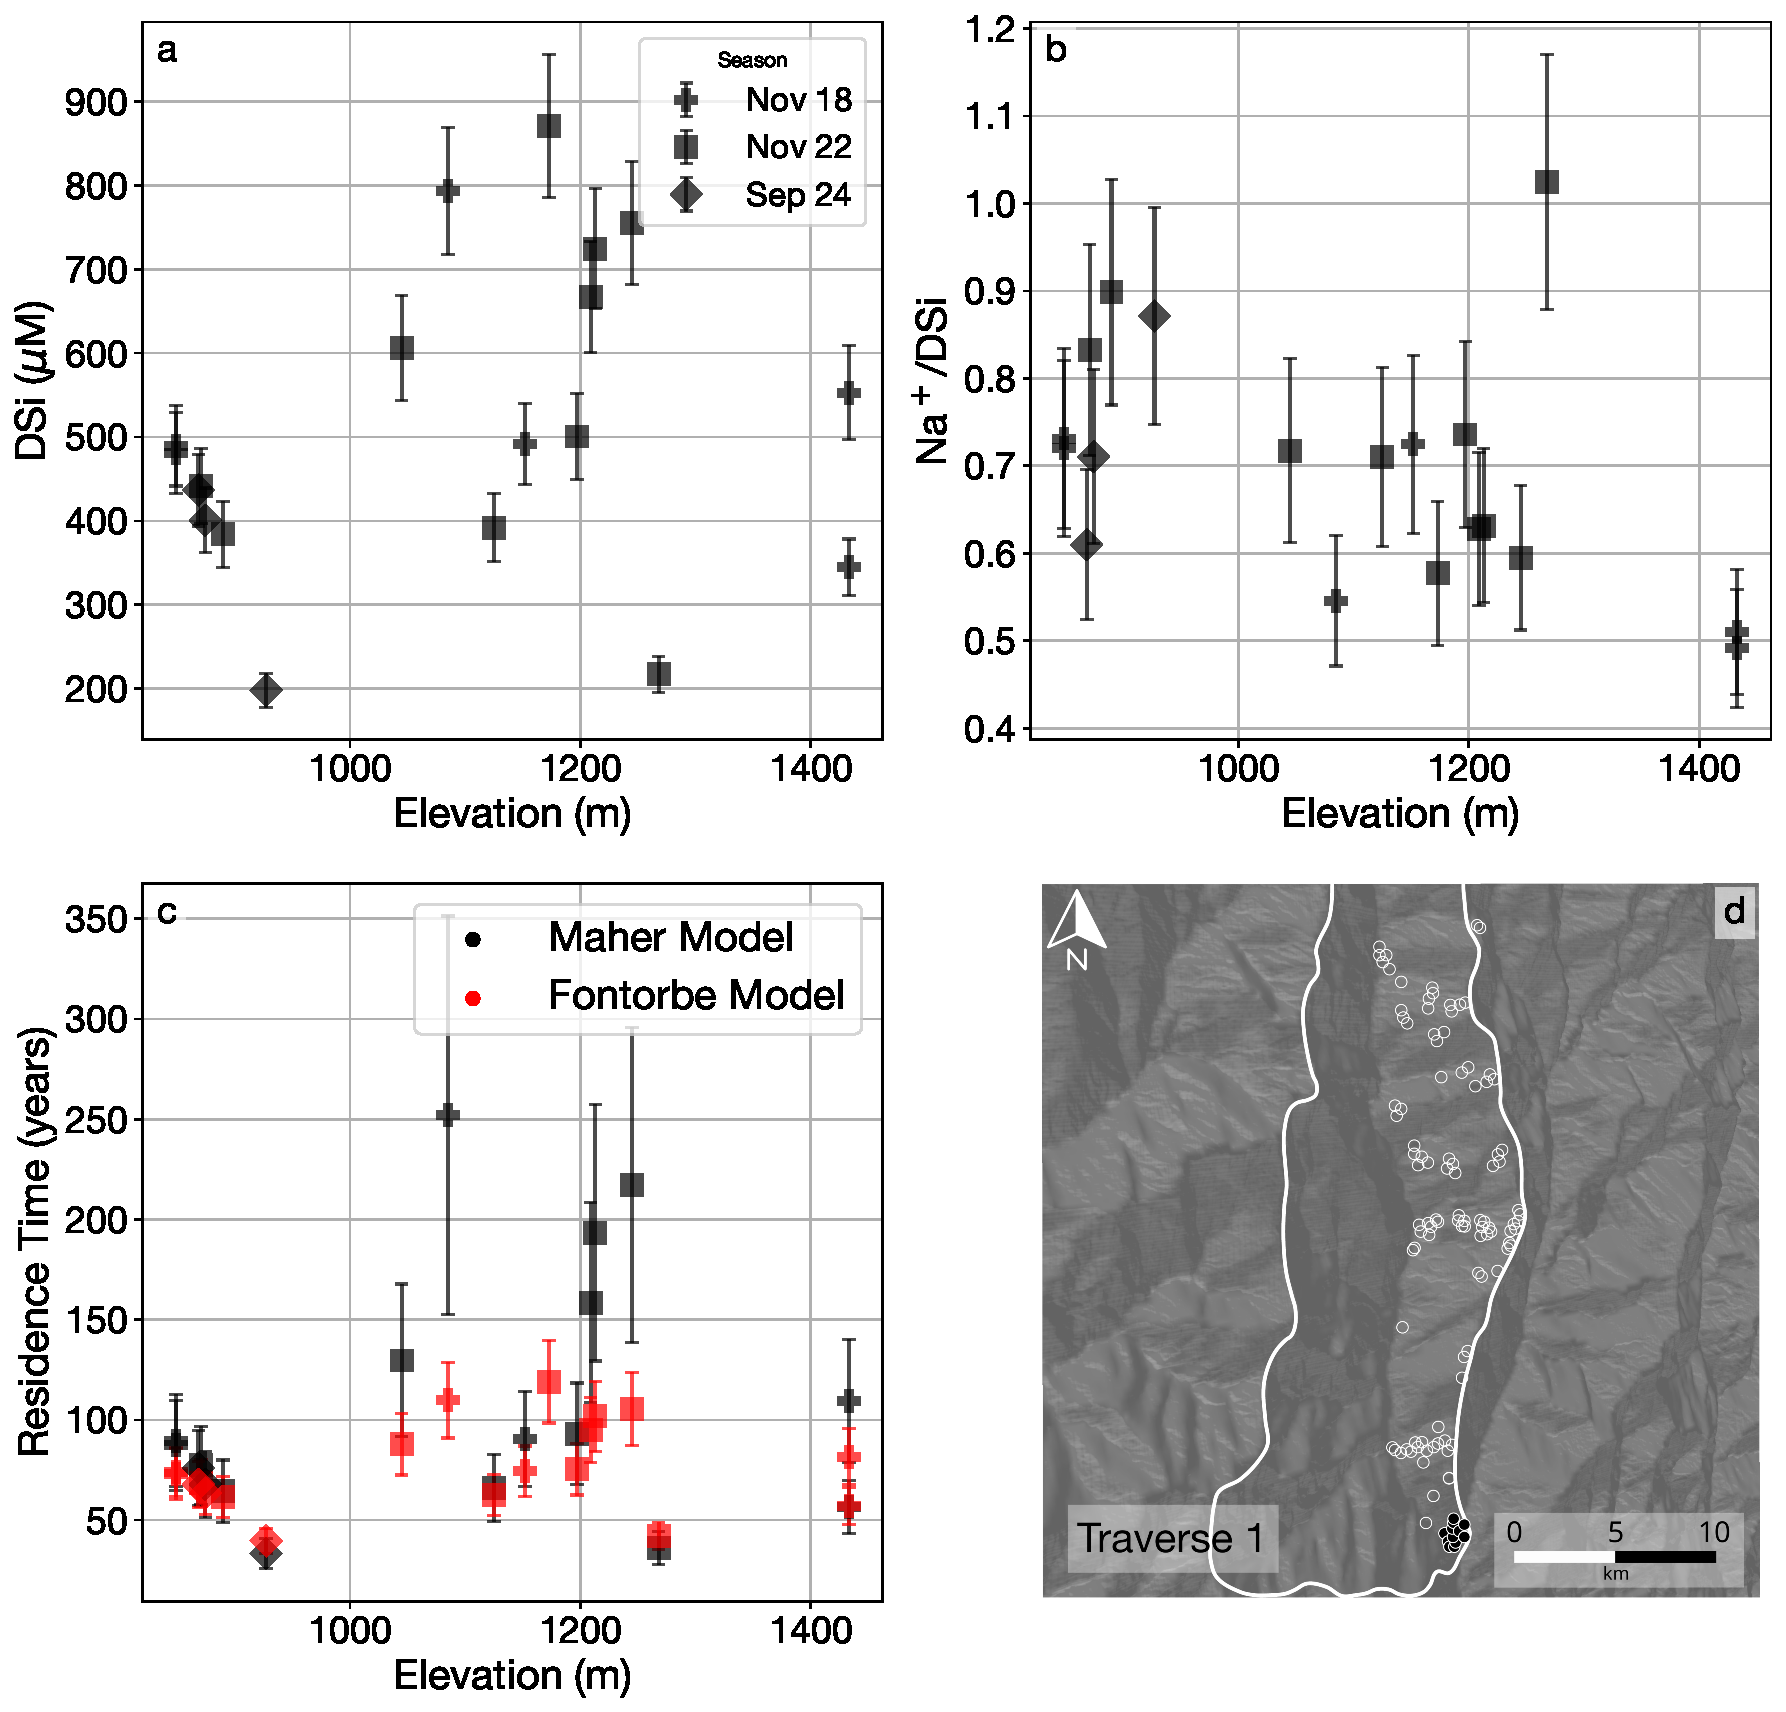
\includegraphics[width=0.9\textwidth]{Traverse_1_summary.pdf}
    \caption{(a) Dissolved silica concentration against elevation for Traverse 2. Error bars reflect Monte Carlo error propagation. Different markers represent different seasons. (b) Na/DSi ratio against elevation. (c) Residence time estimates from the Fontorbe (red) and Maher model (black). (d) Spatial extent of Traverse 1 samples in the catchment. DEM data from NASA ASTER (ref)}
    \label{fig:trav1}
\end{figure}

\FloatBarrier

Concentration of dissolved silica (DSi) in the springs sampled in Traverse 1 is at a maximum for the whole catchment. There is no clear trend of increasing DSi concentration but there is a potentially resolvable increase in Na/DSi with decreasing elevation. The Fontorbe model predicts a peak of $\approx$ 100 years, while the Maher model predicts a much higher residence time of $\approx$ 300 years. 




\subsection{Traverse 2}

\begin{figure}[h]
    \centering
        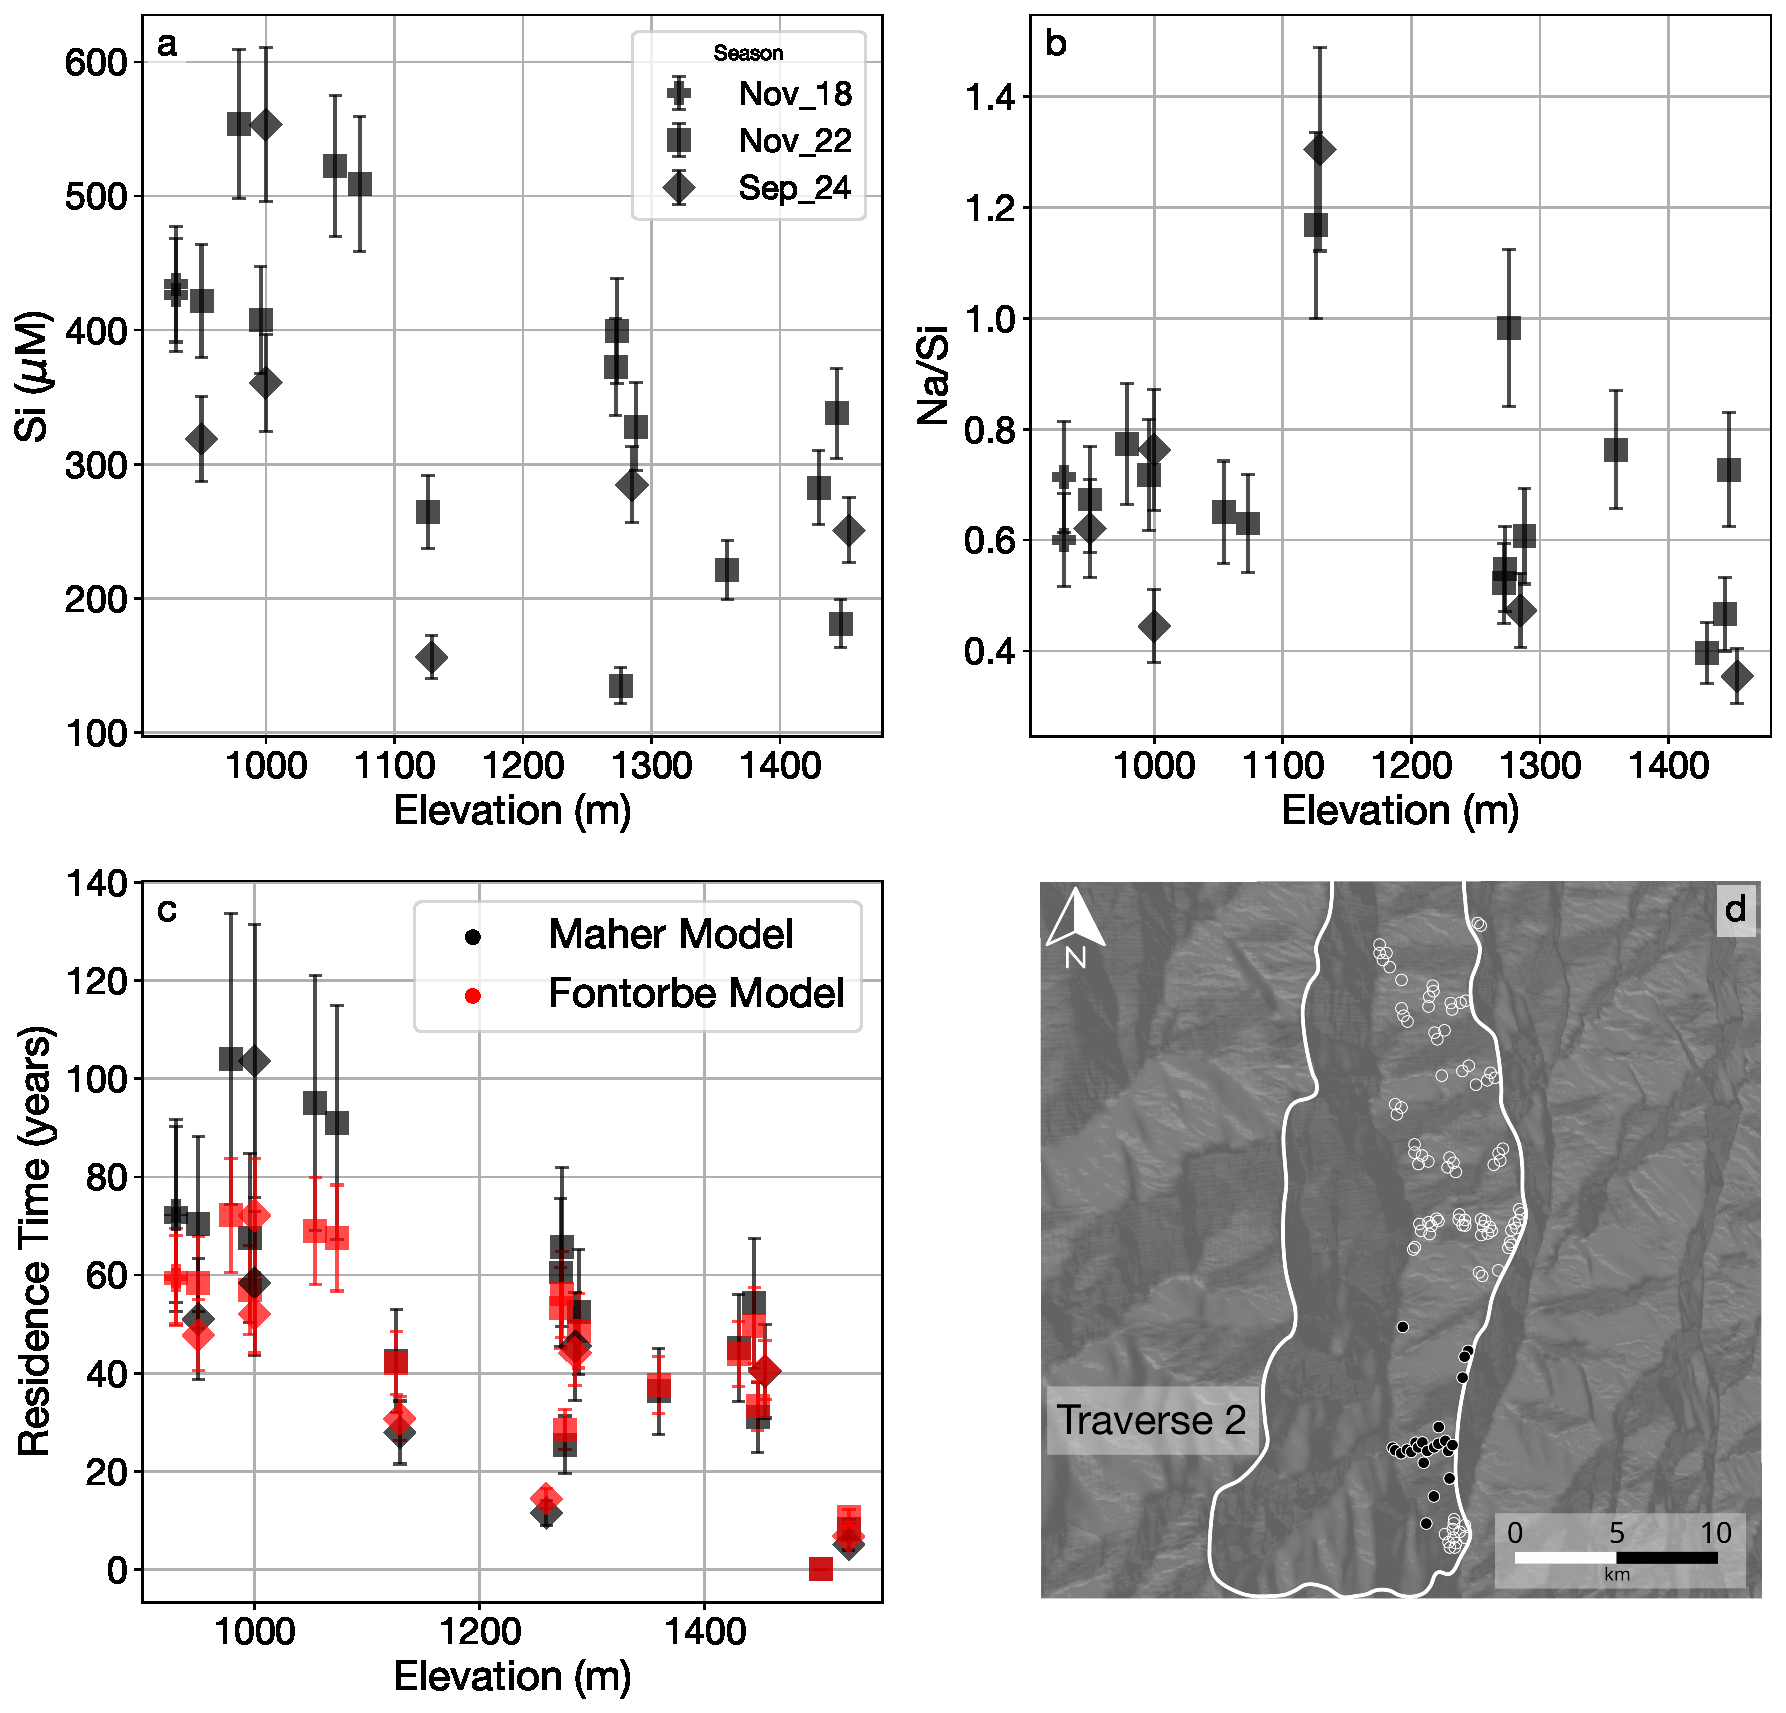
\includegraphics[width=0.9\textwidth]{Traverse_2_summary.pdf}
    \caption{(a) Dissolved silica concentration against elevation for Traverse 2. Error bars reflect Monte Carlo error propagation. Different markers represent different seasons. (b) Na/DSi ratio against elevation. (c) Residence time estimates from the Fontorbe (red) and Maher model (black). (d) Spatial extent of Traverse 2 samples in the catchment. DEM data from NASA ASTER (ref)}
    \label{fig:trav2}
\end{figure}

\FloatBarrier

Dissolved silica concentration shows a clear increase in concentration with decreasing elevation. There is no resolvable trend with Na/DSi and elevation, nor with different seasons when it was collected. Residence times are generally lower than those in Traverse 1, but both showcase a clear trend of higher residence times at lower elevations. The Fontorbe model predicts generally older times than the Maher model at higher elevations, and younger times at lower elevations. 




\subsection{Traverse 3}

\begin{figure}[h]
    \centering
        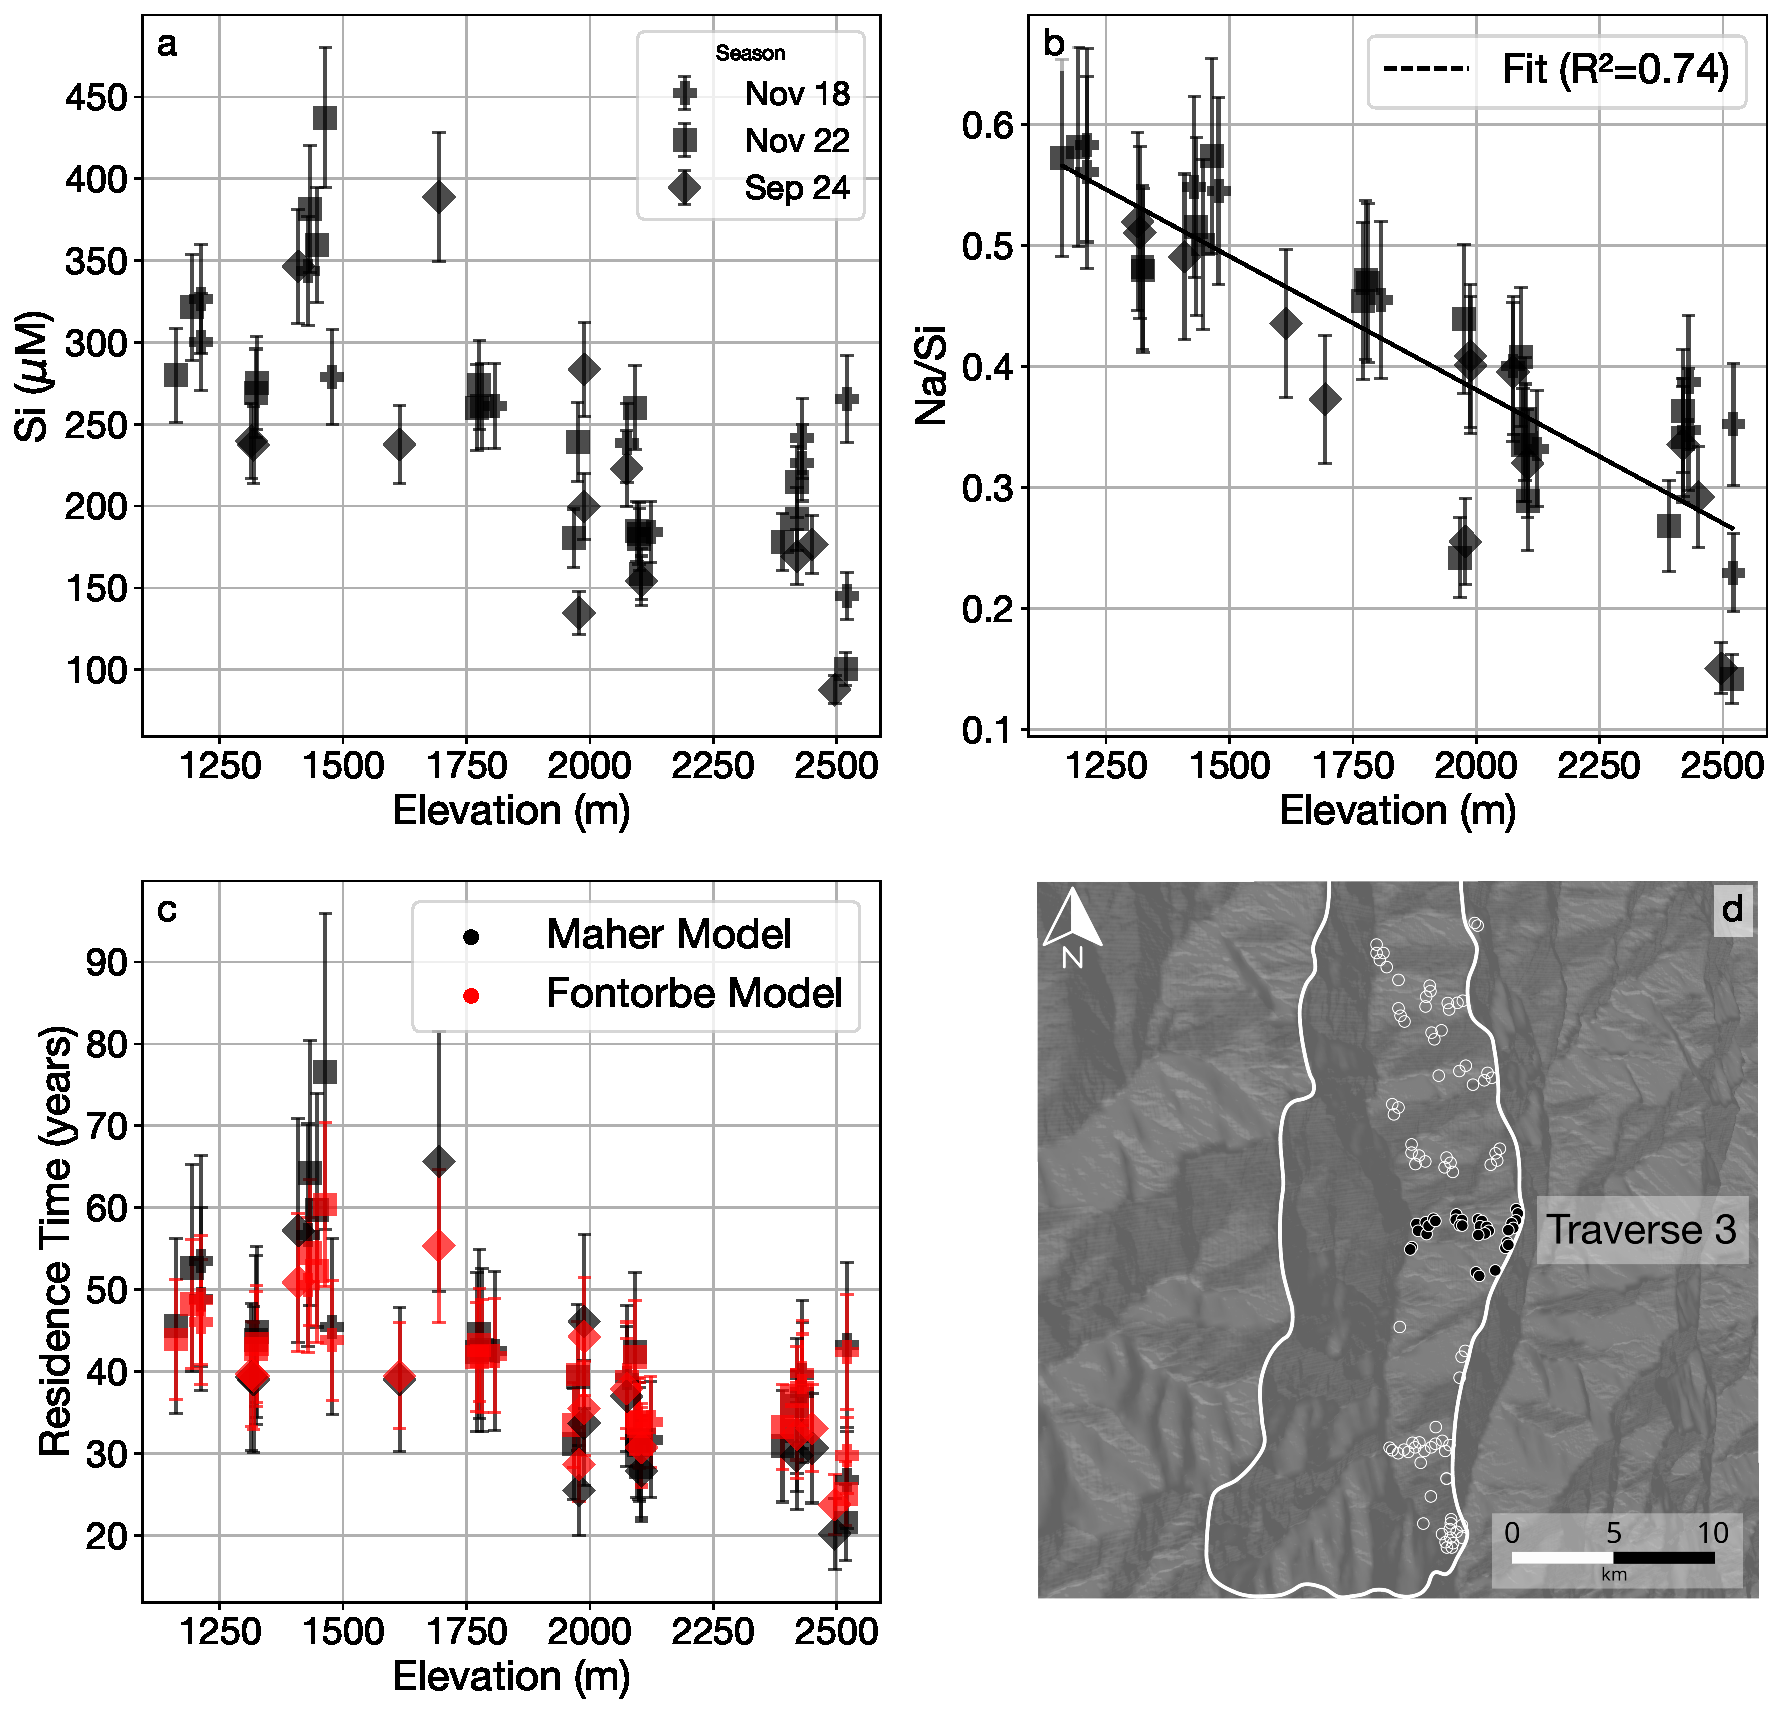
\includegraphics[width=0.9\textwidth]{Traverse_3_summary.pdf}
    \caption{(a) Dissolved silica concentration against elevation for Traverse 3. Error bars reflect Monte Carlo error propagation. Different markers represent different seasons. (b) Na/DSi ratio against elevation. (c) Residence time estimates from the Fontorbe (red) and Maher model (black). (d) Spatial extent of Traverse 3 samples in the catchment. DEM data from NASA ASTER (ref)}
    \label{fig:trav3}
\end{figure}

\FloatBarrier
As elevation decreases, dissolved silica concentration increases in Traverse 3. There is a potential dip at the lowermost elevation sampled. Na/DSi increases with decreasing elevation, consistent between different sampling seasons. Estimated residence times increase as elevation decreases, peaking at $\approx$ 50 years for the Maher model. This peak occurs at the same elevation as the highest DSi concentration.



\subsection{Traverse 4}

Traverse 4 is undersampled compared to the other traverses. DSi increases with decreasing elevation as seen in some of the previous traverses. There is no discernable trend with Na/DSi. Residence times also increase with decreasing elevation as in the previous two traverses, with the Maher model predicting younger times at the highest elevations, and older times at the lowest elevations. The highest residence times predicted are $\approx$ 35 years.

\begin{figure}[h]
    \centering
        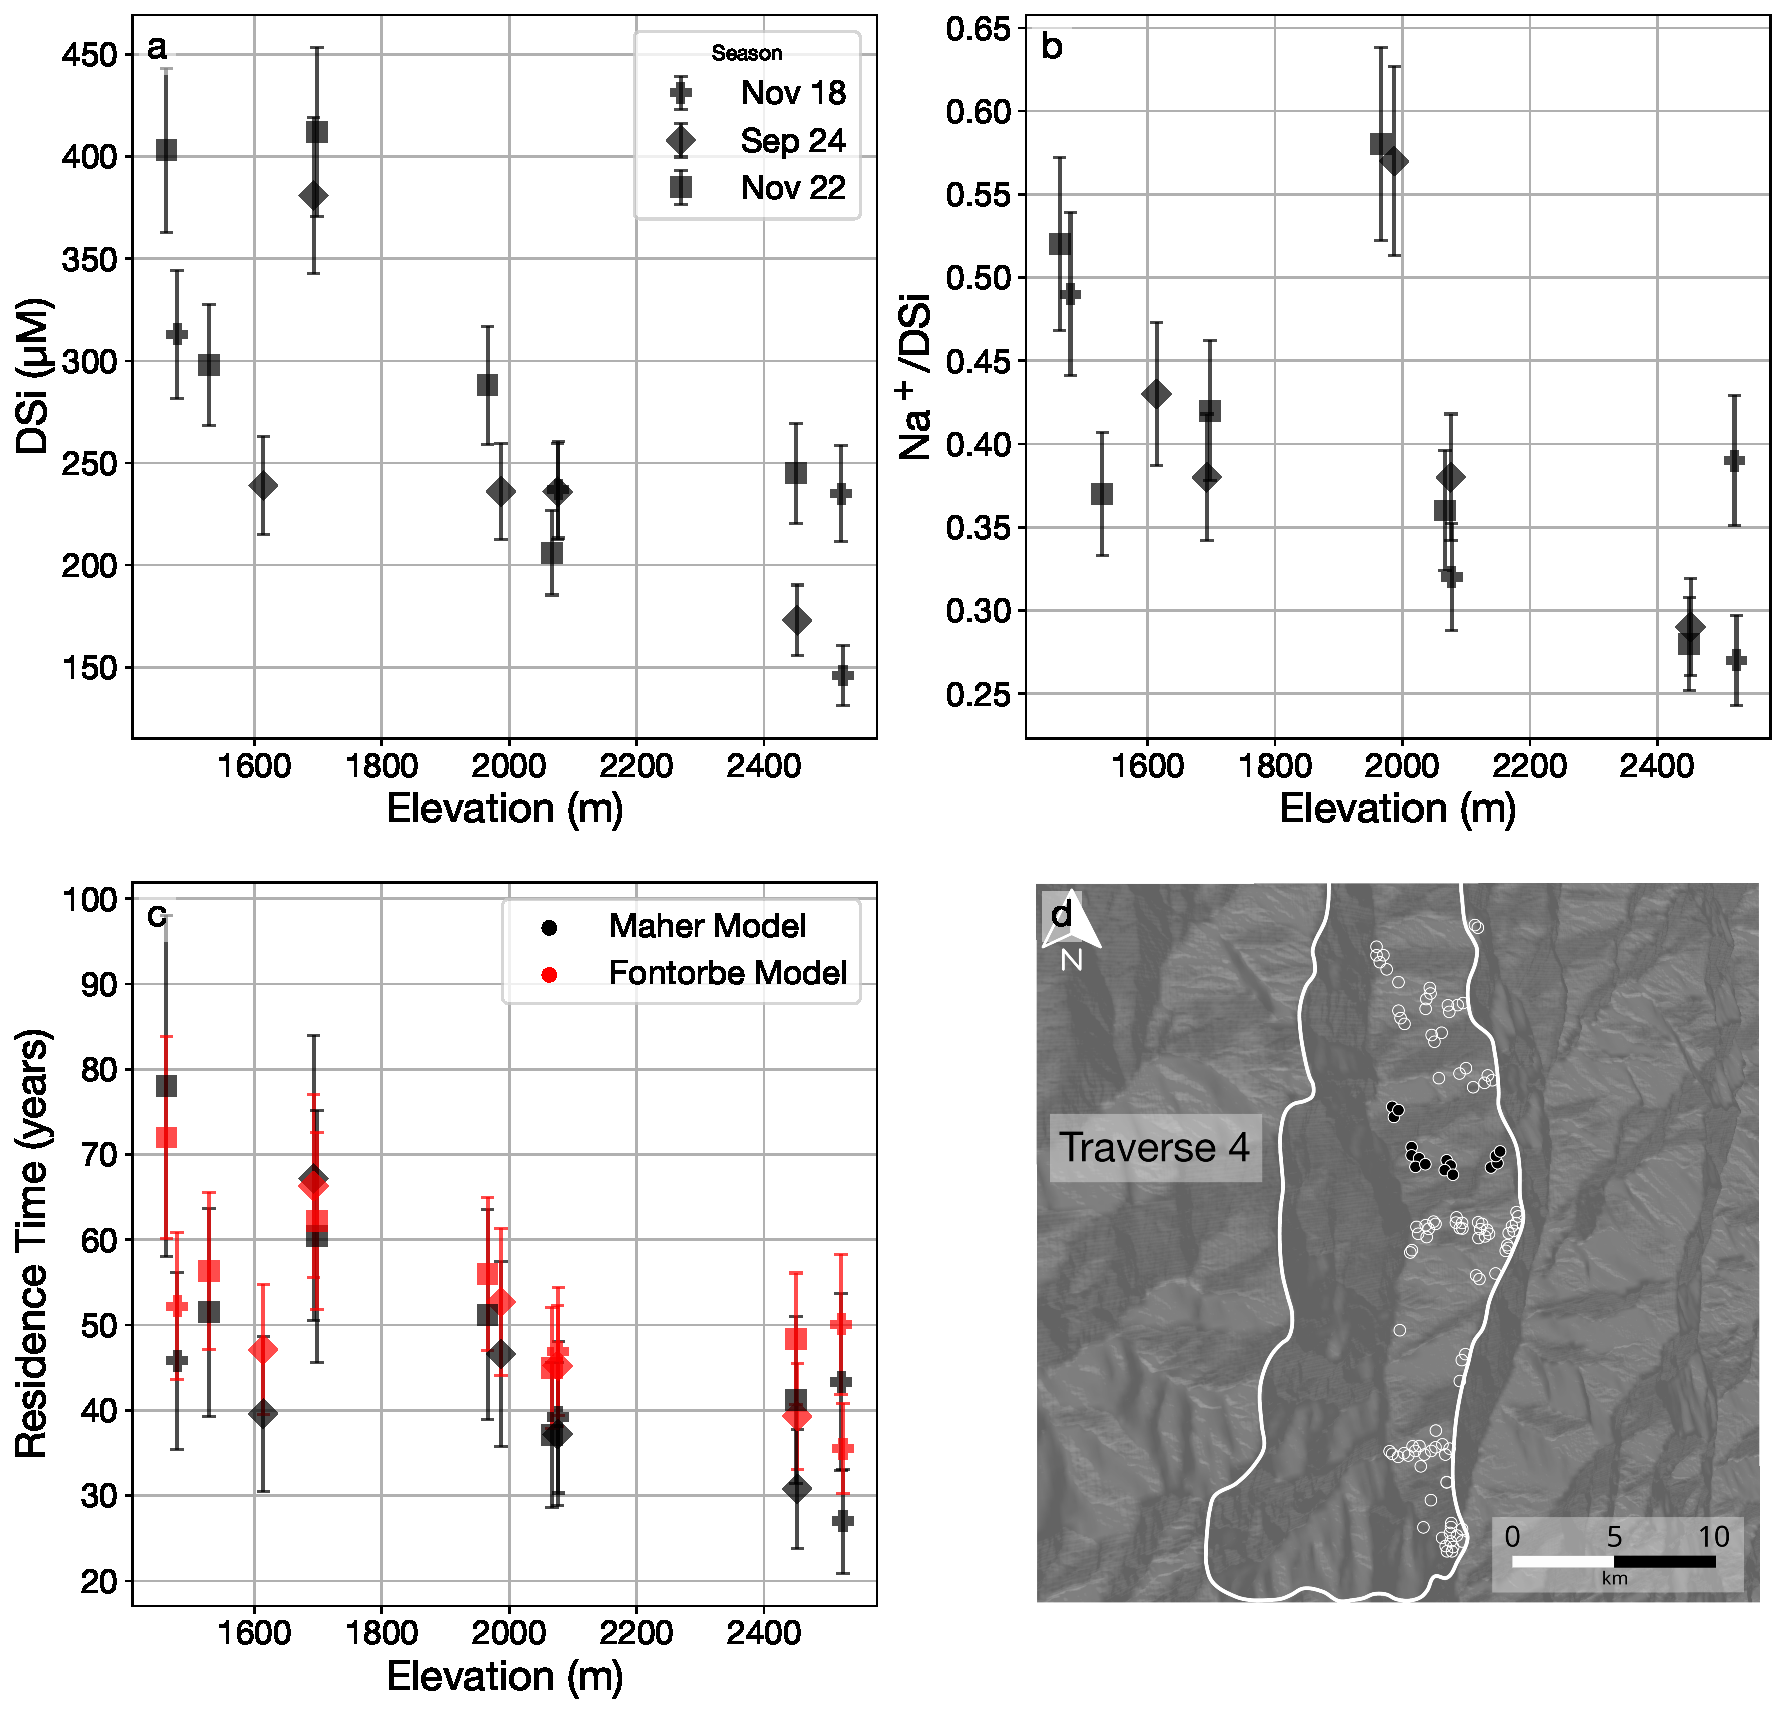
\includegraphics[width=0.9\textwidth]{Traverse_4_summary.pdf}
    \caption{(a) Dissolved silica concentration against elevation for Traverse 4. Error bars reflect Monte Carlo error propagation. Different markers represent different seasons. (b) Na/DSi ratio against elevation. (c) Residence time estimates from the Fontorbe (red) and Maher model (black). (d) Spatial extent of Traverse 4 samples in the catchment. DEM data from NASA ASTER (ref)}
    \label{fig:trav4}
\end{figure}

\FloatBarrier


\subsection{Traverse 5}

\begin{figure}[h]
    \centering
        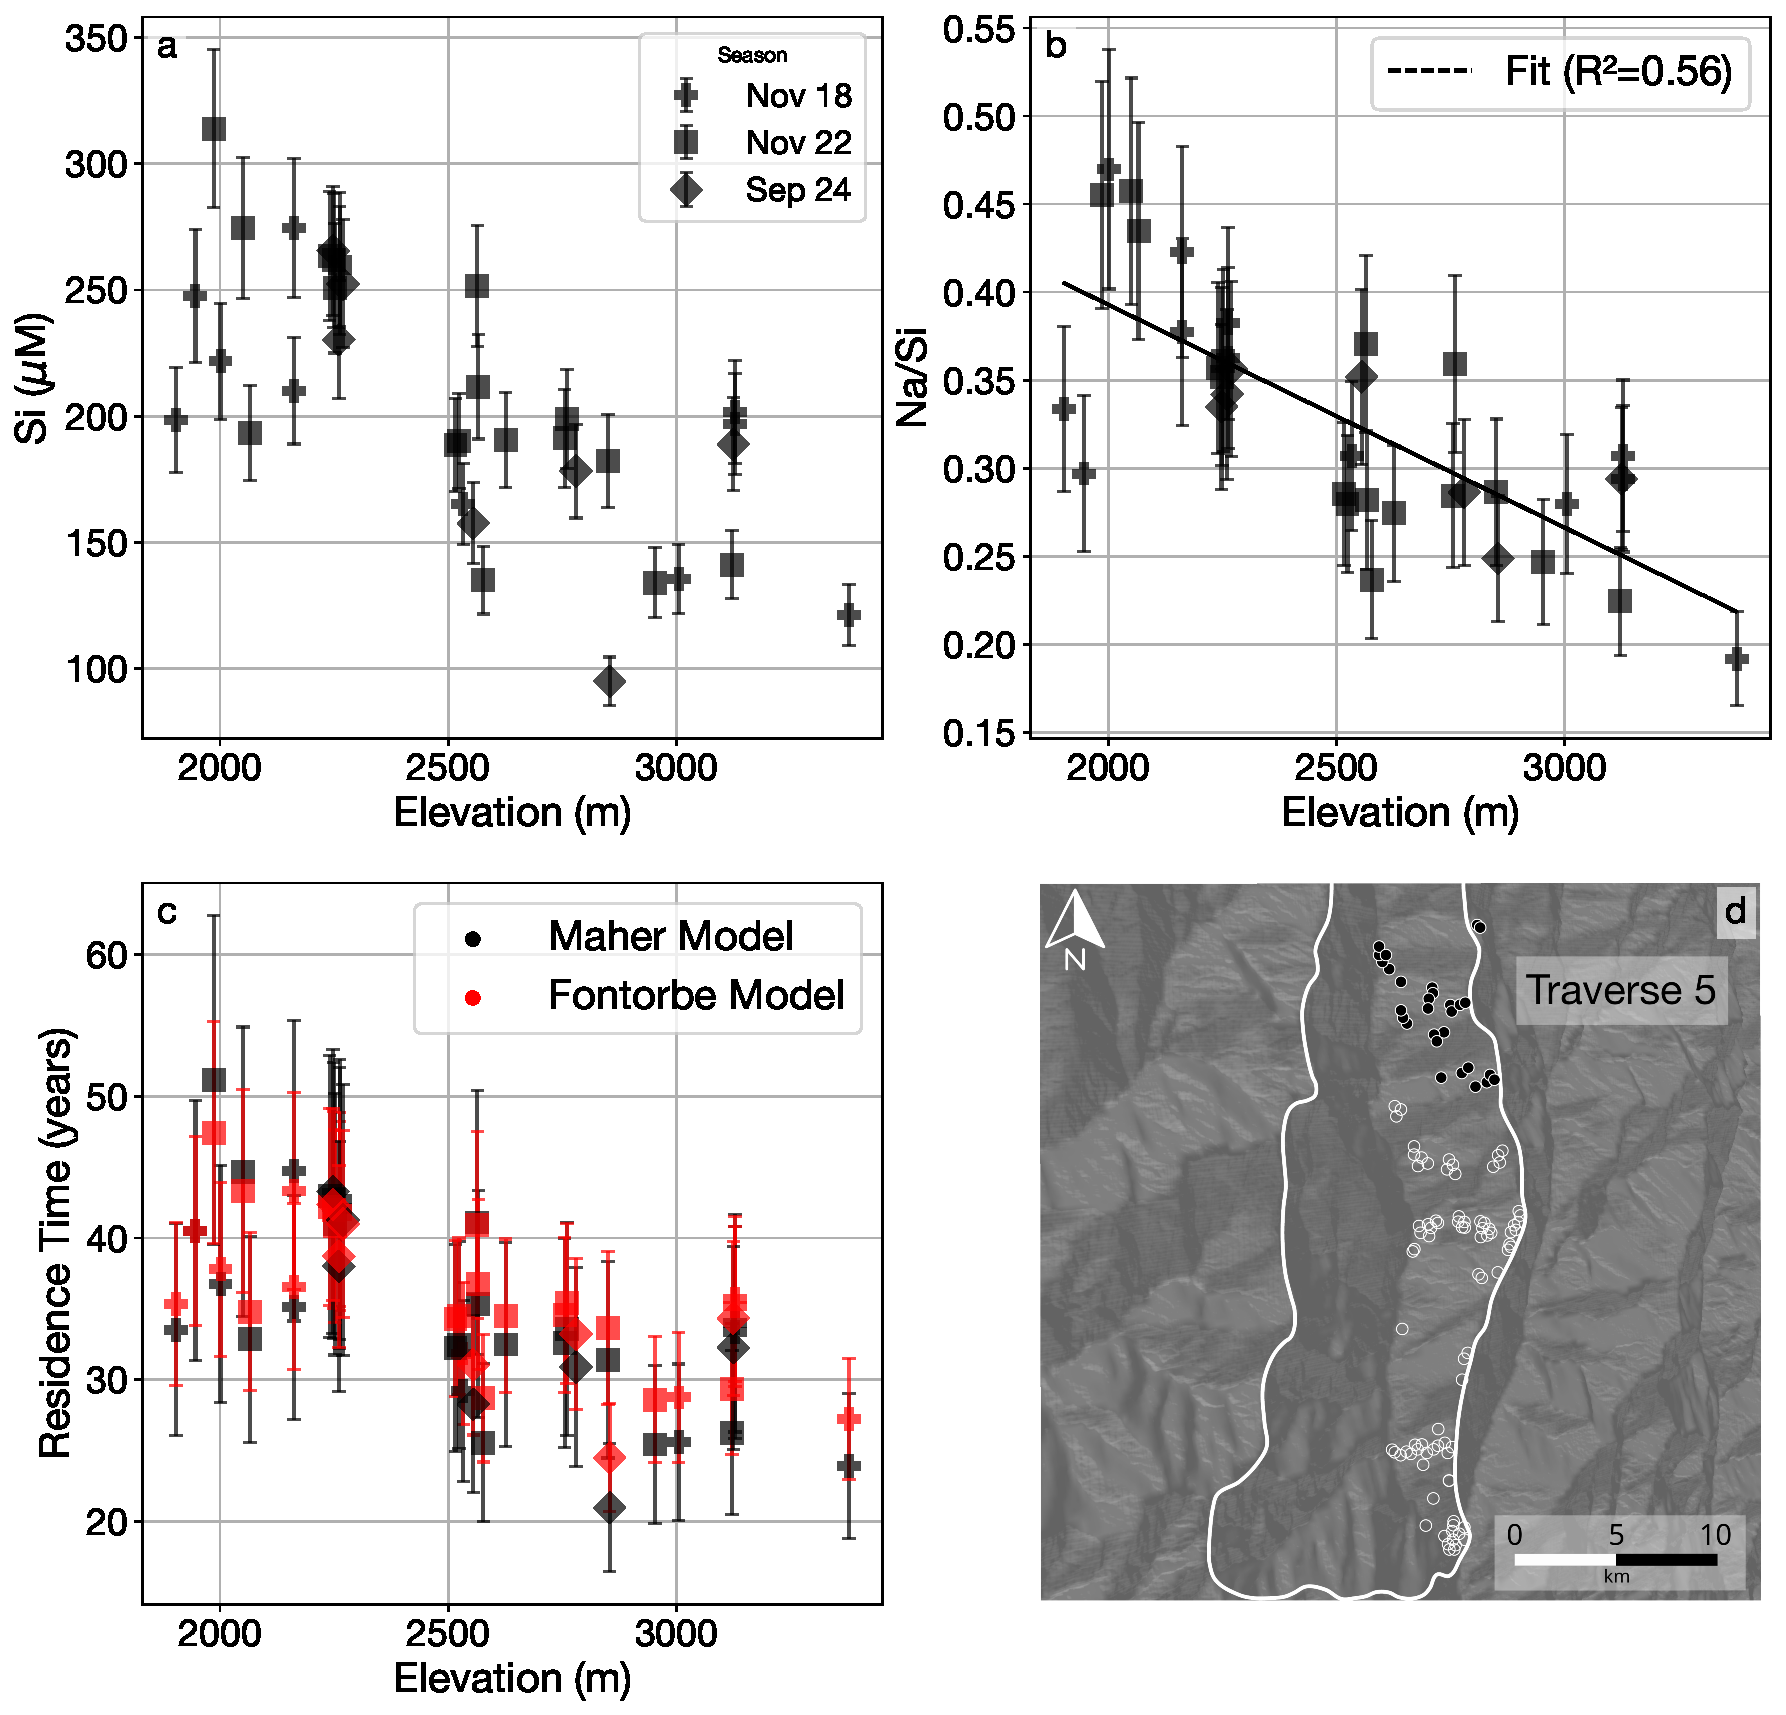
\includegraphics[width=0.9\textwidth]{Traverse_5_summary.pdf}
    \caption{(a) Dissolved silica concentration against elevation for Traverse 5. Error bars reflect Monte Carlo error propagation. Different markers represent different seasons. (b) Na/DSi ratio against elevation. (c) Residence time estimates from the Fontorbe (red) and Maher model (black). (d) Spatial extent of Traverse 5 samples in the catchment. DEM data from NASA ASTER (ref)}
    \label{fig:trav5}
\end{figure}

\FloatBarrier

Traverse 5 is highly sampled and sits at the highest elevation of the whole catchment. DSi concentration increases with decreasing elevation but there is scatter in the data. Na/DSi similarly shows a trend of increasing ratio with decreasing elevation, and it is replicated between different seasons, with considerable scatter. Residence times increase with decreasing elevation, and are the lowest predicted in the catchments.

\newpage

\begin{landscape}

% add to TOC
\addcontentsline{toc}{subsection}{5.6 \phantom{ei} Results Table}

    {\footnotesize
\begin{longtable}{l l l l l l l l l l l l l}

    % Caption should be here, before any rows
    \caption{Summary of results from each traverse. * - All spring elemental concentrations are given after the rain and hydrothermal correction detailed in the Methods, aside from the chloride concentration. ** - Rain samples are displayed as measured, not corrected. Standard deviation of residence time corresponds to Monte Carlo propagated uncertainty} 
    \label{tab:results_table} \\

    
    \hline
    \multicolumn{13}{c}{\textbf{Spring Samples}} \\
    \hline
    \textbf{Sample ID}  &  \textbf{Season}  &  \textbf{Traverse}  &  \textbf{Elevation}  &  \textbf{Cl$^-$*}  &  \textbf{DSi}  &  \textbf{Na$^{2+}$}  &  \textbf{K$^{+}$}  &  \textbf{Ca$^{2+}$}  &  \textbf{Sr$^{2+}$}  &  \textbf{Na$^{+}$/DSi}  &  \textbf{T$_{\text{\textbf{Fontorbe}}} \pm 1\sigma$ }  &  \textbf{T$_{\text{\textbf{Maher}}} \pm 1\sigma$} \\
    \hline
      &   &   &  \textbf{m}  &  \multicolumn{5}{c}{\hspace{-0.35cm}\rule{2.5cm}{0.8pt} \hspace{0.3cm}\textbf{ $\mu$M } \hspace{0.3cm} \rule{2.5cm}{0.8pt}} & \multicolumn{1}{l}{\textbf{nM}} &  &  \multicolumn{2}{c}{\textbf{Years}} \\
    \hline
    \endfirsthead
    
    \hline
    \textbf{Sample ID}  &  \textbf{Season}  &  \textbf{Traverse}  &  \textbf{Elevation}  &  \textbf{Cl$^-$*}  &  \textbf{DSi}  &  \textbf{Na$^{2+}$}  &  \textbf{K$^{+}$}  &  \textbf{Ca$^{2+}$}  &  \textbf{Sr$^{2+}$}  &  \textbf{Na$^{+}$/DSi}  & \textbf{T$_{\text{\textbf{Fontorbe}}} \pm 1\sigma$ }  &  \textbf{T$_{\text{\textbf{Maher}}} \pm 1\sigma$} \\
    \hline
      &   &   &  \textbf{m}  &  \multicolumn{5}{c}{\hspace{-0.35cm}\rule{2.5cm}{0.8pt} \hspace{0.3cm}\textbf{ $\mu$M } \hspace{0.3cm} \rule{2.5cm}{0.8pt}} & \multicolumn{1}{l}{\textbf{nM}} &  &  \multicolumn{2}{c}{\textbf{Years}} \\
    \hline
    \endhead
    \hline
    \endfoot
    \hline
    NEP24-001 & Sep 24 & Traverse 1 & 928 & 93 & 207 & 184 & 6 & 86 & 875 & 0.89 & 41.9 $\pm$ 6.6 & 33.6 $\pm$ 7.6 \\
    NEP22-87 & Nov 22 & Traverse 1 & 1270 & 223 & 214 & 196 & 24 & 195 & 802 & 0.92 & 44.3 $\pm$ 7.0 & 36.2 $\pm$ 8.4 \\
    MKS 1B & Nov 18 & Traverse 1 & 1432 & 25 & 295 & 180 & 11 & 22 & 250 & 0.61 & 60.3 $\pm$ 9.9 & 57.4 $\pm$ 14.0 \\
    NEP22-86 & Nov 22 & Traverse 1 & 1124 & 54 & 355 & 304 & 25 & 35 & 75 & 0.86 & 66.4 $\pm$ 10.8 & 67.5 $\pm$ 16.6 \\
    NEP22-2 & Nov 22 & Traverse 1 & 890 & 93 & 371 & 396 & 47 & 182 & 337 & 1.07 & 65.1 $\pm$ 10.4 & 65.4 $\pm$ 16.6 \\
    NEP22-1 & Nov 22 & Traverse 1 & 871 & 81 & 396 & 335 & 51 & 965 & 296 & 0.85 & 72.2 $\pm$ 12.0 & 78.4 $\pm$ 20.1 \\
    NEP22-85 & Nov 22 & Traverse 1 & 1195 & 2 & 446 & 411 & 19 & 87 & 192 & 0.92 & 79.7 $\pm$ 13.3 & 95.0 $\pm$ 25.1 \\
    NEP24-003 & Sep 24 & Traverse 1 & 876 & 86 & 446 & 289 & 68 & 179 & 246 & 0.65 & 67.2 $\pm$ 10.9 & 68.8 $\pm$ 17.0 \\
    NEP24-002 & Sep 24 & Traverse 1 & 868 & 100 & 456 & 295 & 60 & 832 & 252 & 0.65 & 71.9 $\pm$ 11.7 & 77.8 $\pm$ 20.2 \\
    MKS-3 & Nov 18 & Traverse 1 & 1152 & 7 & 478 & 341 & 48 & 96 & 590 & 0.71 & 78.7 $\pm$ 13.0 & 92.4 $\pm$ 23.9 \\
    MKS-24 & Nov 18 & Traverse 1 & 850 & 49 & 479 & 333 & 92 & 1085 & 463 & 0.7 & 77.2 $\pm$ 12.8 & 89.1 $\pm$ 23.6 \\
    MKS-1 & Nov 18 & Traverse 1 & 1433 & 37 & 583 & 343 & 20 & 99 & 544 & 0.59 & 86.4 $\pm$ 14.0 & 112.7 $\pm$ 30.0 \\
    NEP22-81 & Nov 22 & Traverse 1 & 1207 & 11 & 613 & 455 & 32 & 76 & 214 & 0.74 & 100.5 $\pm$ 16.4 & 164.9 $\pm$ 51.5 \\
    NEP22-80 & Nov 22 & Traverse 1 & 1046 & 6 & 666 & 472 & 31 & 83 & 267 & 0.71 & 92.3 $\pm$ 15.2 & 131.9 $\pm$ 38.6 \\
    NEP22-82 & Nov 22 & Traverse 1 & 1212 & 13 & 705 & 464 & 51 & 95 & 276 & 0.66 & 108.0 $\pm$ 17.8 & 206.2 $\pm$ 73.4 \\
    NEP22-83 & Nov 22 & Traverse 1 & 1244 & 4 & 766 & 407 & 50 & 130 & 327 & 0.53 & 111.5 $\pm$ 18.9 & 230.6 $\pm$ 94.8 \\
    MKS-2 & Nov 18 & Traverse 1 & 1083 & 8 & 821 & 417 & 55 & 124 & 258 & 0.51 & 116.6 $\pm$ 19.4 & 275.0 $\pm$ 118.4 \\
    \specialrule{0.2pt}{1pt}{1pt}
    NEP22-79 & Nov 22 & Traverse 2 & 1277 & 306 & 122 & 120 & 7 & 77 & 267 & 0.98 & 34.1 $\pm$ 5.3 & 25.6 $\pm$ 5.8 \\
    NEP22-63 & Nov 22 & Traverse 2 & 1447 & 152 & 190 & 136 & 11 & 16 & 498 & 0.72 & 39.9 $\pm$ 6.3 & 31.5 $\pm$ 7.0 \\
    NEP24-065 & Sep 24 & Traverse 2 & 1129 & 259 & 190 & 211 & 45 & 136 & 296 & 1.11 & 36.9 $\pm$ 5.7 & 28.4 $\pm$ 6.4 \\
    NEP22-66 & Nov 22 & Traverse 2 & 1359 & 126 & 241 & 160 & 11 & 3 & 31 & 0.66 & 45.0 $\pm$ 6.9 & 37.1 $\pm$ 8.5 \\
    NEP24-062 & Sep 24 & Traverse 2 & 1452 & 82 & 243 & 97 & 16 & 0 & 176 & 0.4 & 48.7 $\pm$ 7.7 & 41.4 $\pm$ 9.4 \\
    NEP22-65 & Nov 22 & Traverse 2 & 1429 & 59 & 267 & 122 & 16 & 2 & 137 & 0.46 & 52.8 $\pm$ 8.6 & 46.5 $\pm$ 10.5 \\
    NEP24-063 & Sep 24 & Traverse 2 & 1285 & 110 & 277 & 134 & 14 & 68 & 253 & 0.48 & 53.2 $\pm$ 8.7 & 47.1 $\pm$ 11.0 \\
    NEP24-067 & Sep 24 & Traverse 2 & 1000 & 58 & 298 & 295 & 39 & 102 & 377 & 0.99 & 62.6 $\pm$ 10.2 & 61.1 $\pm$ 14.9 \\
    NEP22-67 & Nov 22 & Traverse 2 & 1125 & 236 & 301 & 280 & 47 & 214 & 481 & 0.93 & 50.3 $\pm$ 8.1 & 43.5 $\pm$ 10.4 \\
    NEP24-068 & Sep 24 & Traverse 2 & 949 & 95 & 309 & 221 & 38 & 353 & 678 & 0.72 & 56.8 $\pm$ 9.3 & 52.2 $\pm$ 12.4 \\
    NEP22-68 & Nov 22 & Traverse 2 & 1288 & 113 & 311 & 239 & 13 & 85 & 230 & 0.77 & 58.2 $\pm$ 9.5 & 54.3 $\pm$ 13.2 \\
    MKS-10 & Nov 18 & Traverse 2 & 930 & 33 & 355 & 263 & 49 & 479 & 969 & 0.74 & 71.1 $\pm$ 11.7 & 76.3 $\pm$ 19.7 \\
    NEP22-71 & Nov 22 & Traverse 2 & 996 & 126 & 359 & 286 & 26 & 179 & 283 & 0.8 & 68.5 $\pm$ 11.2 & 71.3 $\pm$ 17.7 \\
    NEP22-64 & Nov 22 & Traverse 2 & 1442 & 102 & 371 & 171 & 17 & 28 & 366 & 0.46 & 59.5 $\pm$ 9.7 & 56.2 $\pm$ 13.6 \\
    NEP22-77 & Nov 22 & Traverse 2 & 1273 & 38 & 371 & 192 & 58 & 58 & 201 & 0.52 & 67.5 $\pm$ 11.2 & 69.4 $\pm$ 17.2 \\
    MKS 10B & Nov 18 & Traverse 2 & 929 & 36 & 386 & 384 & 55 & 511 & 1128 & 0.99 & 70.5 $\pm$ 11.6 & 75.0 $\pm$ 18.8 \\
    NEP22-78 & Nov 22 & Traverse 2 & 1270 & 40 & 393 & 188 & 24 & 32 & 184 & 0.48 & 63.7 $\pm$ 10.3 & 62.9 $\pm$ 15.3 \\
    NEP22-76 & Nov 22 & Traverse 2 & 1074 & 112 & 470 & 321 & 26 & 429 & 404 & 0.68 & 80.7 $\pm$ 13.4 & 97.9 $\pm$ 27.8 \\
    NEP22-70 & Nov 22 & Traverse 2 & 950 & 61 & 473 & 294 & 40 & 643 & 1250 & 0.62 & 70.0 $\pm$ 11.4 & 74.2 $\pm$ 18.6 \\
    NEP22-75 & Nov 22 & Traverse 2 & 1052 & 117 & 519 & 329 & 37 & 363 & 443 & 0.63 & 82.4 $\pm$ 13.7 & 101.5 $\pm$ 27.3 \\
    NEP22-73 & Nov 22 & Traverse 2 & 979 & 42 & 639 & 456 & 68 & 224 & 837 & 0.71 & 86.6 $\pm$ 14.2 & 113.3 $\pm$ 31.0 \\
    \specialrule{0.2pt}{1pt}{1pt}
    NEP24-014 & Sep 24 & Traverse 3 & 2496 & 2 & 90 & 12 & 2 & 3 & 34 & 0.13 & 28.3 $\pm$ 4.3 & 20.3 $\pm$ 4.4 \\
    NEP22-9 & Nov 22 & Traverse 3 & 2522 & 2 & 99 & 11 & 2 & 5 & 42 & 0.11 & 29.9 $\pm$ 4.5 & 21.7 $\pm$ 4.7 \\
    NEP24-016 & Sep 24 & Traverse 3 & 1979 & 0 & 140 & 35 & 11 & 27 & 141 & 0.25 & 34.0 $\pm$ 5.3 & 25.5 $\pm$ 5.7 \\
    NEP24-015 & Sep 24 & Traverse 3 & 2101 & 7 & 160 & 61 & 8 & 0 & 200 & 0.38 & 36.6 $\pm$ 5.7 & 28.0 $\pm$ 6.2 \\
    NEP22-19 & Nov 22 & Traverse 3 & 2097 & 9 & 171 & 66 & 7 & 6 & 244 & 0.39 & 40.3 $\pm$ 6.3 & 31.8 $\pm$ 7.2 \\
    NEP22-13 & Nov 22 & Traverse 3 & 2098 & 9 & 172 & 71 & 8 & 6 & 249 & 0.41 & 40.1 $\pm$ 6.2 & 31.7 $\pm$ 7.2 \\
    NEP24-034 & Sep 24 & Traverse 3 & 2415 & 12 & 182 & 50 & 9 & 0 & 215 & 0.27 & 38.3 $\pm$ 6.2 & 29.8 $\pm$ 6.8 \\
    NEP22-46 & Nov 22 & Traverse 3 & 2555 & 3 & 183 & 65 & 11 & 61 & 159 & 0.36 & 37.3 $\pm$ 5.8 & 28.7 $\pm$ 6.5 \\
    NEP22-17 & Nov 22 & Traverse 3 & 2102 & 12 & 185 & 63 & 7 & 2 & 224 & 0.34 & 39.9 $\pm$ 6.2 & 31.5 $\pm$ 7.2 \\
    NEP22-20 & Nov 22 & Traverse 3 & 2104 & 7 & 186 & 53 & 7 & 0 & 113 & 0.28 & 37.0 $\pm$ 5.8 & 28.5 $\pm$ 6.4 \\
    NEP22-15 & Nov 22 & Traverse 3 & 1973 & 5 & 190 & 108 & 9 & 54 & 197 & 0.57 & 47.3 $\pm$ 7.7 & 39.7 $\pm$ 9.1 \\
    NEP22-12 & Nov 22 & Traverse 3 & 2386 & 3 & 192 & 42 & 3 & 15 & 153 & 0.22 & 39.4 $\pm$ 6.1 & 30.9 $\pm$ 7.0 \\
    MKS-6 & Nov 18 & Traverse 3 & 2124 & 9 & 195 & 65 & 8 & 0 & 160 & 0.33 & 40.2 $\pm$ 6.4 & 31.8 $\pm$ 7.2 \\
    NEP24-017 & Sep 24 & Traverse 3 & 1990 & 1 & 196 & 75 & 8 & 25 & 178 & 0.38 & 42.3 $\pm$ 6.6 & 34.0 $\pm$ 7.7 \\
    NEP22-11 & Nov 22 & Traverse 3 & 2418 & 16 & 197 & 90 & 6 & 2 & 206 & 0.46 & 44.3 $\pm$ 6.9 & 36.2 $\pm$ 8.1 \\
    NEP22-16 & Nov 22 & Traverse 3 & 1964 & 1 & 211 & 42 & 8 & 25 & 123 & 0.2 & 39.8 $\pm$ 6.2 & 31.3 $\pm$ 7.0 \\
    NEP22-10 & Nov 22 & Traverse 3 & 2418 & 17 & 217 & 64 & 5 & 0 & 194 & 0.29 & 41.6 $\pm$ 6.5 & 33.3 $\pm$ 7.5 \\
    MKS 5B & Nov 18 & Traverse 3 & 2428 & 14 & 217 & 98 & 12 & 1 & 265 & 0.45 & 47.3 $\pm$ 7.5 & 39.7 $\pm$ 9.0 \\
    MKS-5 & Nov 18 & Traverse 3 & 2434 & 14 & 235 & 79 & 9 & 5 & 217 & 0.34 & 45.6 $\pm$ 7.2 & 37.8 $\pm$ 8.9 \\
    NEP24-011 & Sep 24 & Traverse 3 & 1318 & 11 & 239 & 112 & 14 & 32 & 334 & 0.47 & 47.0 $\pm$ 7.3 & 39.4 $\pm$ 9.0 \\
    NEP24-010 & Sep 24 & Traverse 3 & 1314 & 22 & 240 & 124 & 13 & 39 & 315 & 0.52 & 47.4 $\pm$ 7.6 & 39.8 $\pm$ 9.2 \\
    NEP22-55 & Nov 22 & Traverse 3 & 1772 & 20 & 251 & 119 & 17 & 33 & 319 & 0.47 & 49.9 $\pm$ 7.9 & 42.9 $\pm$ 10.1 \\
    MKS-7 & Nov 18 & Traverse 3 & 1805 & 21 & 257 & 104 & 19 & 32 & 300 & 0.4 & 50.0 $\pm$ 8.1 & 43.0 $\pm$ 10.1 \\
    NEP22-42 & Nov 22 & Traverse 3 & 1325 & 27 & 258 & 137 & 9 & 35 & 351 & 0.53 & 51.8 $\pm$ 8.4 & 45.4 $\pm$ 10.7 \\
    NEP22-58 & Nov 22 & Traverse 3 & 1447 & 8 & 271 & 166 & 14 & 74 & 326 & 0.61 & 62.2 $\pm$ 10.4 & 60.4 $\pm$ 14.5 \\
    NEP22-60 & Nov 22 & Traverse 3 & 1160 & 23 & 279 & 184 & 19 & 63 & 323 & 0.66 & 52.3 $\pm$ 8.4 & 46.0 $\pm$ 10.3 \\
    NEP22-18 & Nov 22 & Traverse 3 & 2091 & 9 & 281 & 101 & 15 & 25 & 362 & 0.36 & 49.7 $\pm$ 7.9 & 42.7 $\pm$ 9.8 \\
    NEP22-53 & Nov 22 & Traverse 3 & 1777 & 20 & 284 & 113 & 17 & 46 & 392 & 0.4 & 51.3 $\pm$ 8.4 & 44.8 $\pm$ 10.6 \\
    NEP22-59 & Nov 22 & Traverse 3 & 1324 & 15 & 291 & 134 & 12 & 30 & 351 & 0.46 & 50.9 $\pm$ 8.2 & 44.2 $\pm$ 10.2 \\
    NEP22-54 & Nov 22 & Traverse 3 & 1779 & 20 & 294 & 112 & 15 & 38 & 387 & 0.38 & 50.1 $\pm$ 8.0 & 43.2 $\pm$ 10.0 \\
    NEP22-45 & Nov 22 & Traverse 3 & 1195 & 24 & 315 & 184 & 6 & 47 & 323 & 0.58 & 57.6 $\pm$ 9.1 & 53.4 $\pm$ 12.6 \\
    MKS 9B & Nov 18 & Traverse 3 & 1214 & 16 & 349 & 192 & 10 & 44 & 384 & 0.55 & 58.5 $\pm$ 9.7 & 54.6 $\pm$ 12.9 \\
    MKS-9 & Nov 18 & Traverse 3 & 1212 & 17 & 354 & 193 & 11 & 47 & 311 & 0.55 & 54.8 $\pm$ 8.7 & 49.4 $\pm$ 11.6 \\
    NEP22-56 & Nov 22 & Traverse 3 & 1433 & 23 & 356 & 209 & 13 & 83 & 401 & 0.59 & 65.0 $\pm$ 10.9 & 65.0 $\pm$ 16.0 \\
    NEP24-038 & Sep 24 & Traverse 3 & 1408 & 20 & 369 & 155 & 19 & 69 & 406 & 0.42 & 60.6 $\pm$ 10.0 & 58.0 $\pm$ 14.3 \\
    MKS-8 & Nov 18 & Traverse 3 & 1430 & 15 & 431 & 190 & 17 & 72 & 408 & 0.44 & 60.3 $\pm$ 10.0 & 57.5 $\pm$ 14.0 \\
    \specialrule{0.2pt}{1pt}{1pt}
    MKS 4B & Nov 18 & Traverse 4 & 2524 & 3 & 146 & 39 & 2 & 1 & 108 & 0.27 & 35.5 $\pm$ 5.3 & 27.0 $\pm$ 6.1 \\
    NEP24-050 & Sep 24 & Traverse 4 & 2452 & 2 & 173 & 51 & 7 & 11 & 141 & 0.29 & 39.3 $\pm$ 6.2 & 30.8 $\pm$ 7.0 \\
    NEP22-48 & Nov 22 & Traverse 4 & 2067 & 3 & 206 & 75 & 7 & 32 & 254 & 0.36 & 45.0 $\pm$ 7.1 & 37.1 $\pm$ 8.5 \\
    MKS-4 & Nov 18 & Traverse 4 & 2521 & 2 & 235 & 92 & 9 & 31 & 207 & 0.39 & 50.1 $\pm$ 8.2 & 43.3 $\pm$ 10.4 \\
    NEP24-052 & Sep 24 & Traverse 4 & 1987 & 0 & 236 & 134 & 17 & 73 & 382 & 0.57 & 52.7 $\pm$ 8.6 & 46.6 $\pm$ 10.9 \\
    NEP24-051 & Sep 24 & Traverse 4 & 2076 & 2 & 236 & 89 & 10 & 25 & 212 & 0.38 & 45.2 $\pm$ 7.1 & 37.2 $\pm$ 8.4 \\
    MKS-13 & Nov 18 & Traverse 4 & 2077 & 2 & 237 & 77 & 9 & 31 & 236 & 0.32 & 46.9 $\pm$ 7.5 & 39.2 $\pm$ 8.9 \\
    NEP24-041 & Sep 24 & Traverse 4 & 1614 & 12 & 239 & 103 & 25 & 17 & 246 & 0.43 & 47.1 $\pm$ 7.6 & 39.6 $\pm$ 9.1 \\
    NEP22-47 & Nov 22 & Traverse 4 & 2450 & 8 & 245 & 68 & 7 & 31 & 169 & 0.28 & 48.4 $\pm$ 7.7 & 41.2 $\pm$ 9.8 \\
    NEP22-49 & Nov 22 & Traverse 4 & 1966 & 5 & 288 & 167 & 13 & 61 & 424 & 0.58 & 56.0 $\pm$ 9.0 & 51.2 $\pm$ 12.3 \\
    NEP22-52 & Nov 22 & Traverse 4 & 1529 & 8 & 298 & 111 & 7 & 20 & 158 & 0.37 & 56.3 $\pm$ 9.2 & 51.5 $\pm$ 12.2 \\
    MKS-12 & Nov 18 & Traverse 4 & 1479 & 9 & 313 & 153 & 29 & 100 & 408 & 0.49 & 52.2 $\pm$ 8.6 & 45.8 $\pm$ 10.4 \\
    NEP24-040 & Sep 24 & Traverse 4 & 1693 & 22 & 381 & 145 & 12 & 86 & 590 & 0.38 & 66.3 $\pm$ 10.7 & 67.2 $\pm$ 16.7 \\
    NEP22-57 & Nov 22 & Traverse 4 & 1462 & 46 & 403 & 211 & 21 & 104 & 661 & 0.52 & 72.0 $\pm$ 11.8 & 78.0 $\pm$ 20.0 \\
    NEP22-50 & Nov 22 & Traverse 4 & 1698 & 21 & 412 & 173 & 22 & 73 & 682 & 0.42 & 62.2 $\pm$ 10.4 & 60.4 $\pm$ 14.8 \\
    \specialrule{0.2pt}{1pt}{1pt}
    NEP24-027 & Sep 24 & Traverse 5 & 2858 & 2 & 105 & 25 & 10 & 11 & 68 & 0.24 & 29.2 $\pm$ 4.4 & 21.1 $\pm$ 4.6 \\
    NEP22-28 & Nov 22 & Traverse 5 & 2954 & 2 & 107 & 30 & 8 & 17 & 92 & 0.28 & 34.1 $\pm$ 5.2 & 25.6 $\pm$ 5.7 \\
    MKS-23 & Nov 18 & Traverse 5 & 3379 & 1 & 124 & 21 & 0 & 5 & 47 & 0.17 & 32.6 $\pm$ 5.0 & 24.2 $\pm$ 5.4 \\
    MKS 21B & Nov 18 & Traverse 5 & 3007 & 4 & 144 & 35 & 9 & 1 & 29 & 0.24 & 34.3 $\pm$ 5.3 & 25.8 $\pm$ 5.7 \\
    NEP24-020 & Sep 24 & Traverse 5 & 2556 & 4 & 150 & 59 & 13 & 26 & 216 & 0.39 & 37.0 $\pm$ 5.8 & 28.5 $\pm$ 6.5 \\
    NEP22-39 & Nov 22 & Traverse 5 & 2523 & 5 & 165 & 53 & 13 & 37 & 182 & 0.32 & 41.0 $\pm$ 6.6 & 32.6 $\pm$ 7.4 \\
    NEP24-028 & Sep 24 & Traverse 5 & 2782 & 2 & 167 & 54 & 17 & 24 & 169 & 0.32 & 39.4 $\pm$ 6.2 & 30.9 $\pm$ 7.0 \\
    MKS-14 & Nov 18 & Traverse 5 & 2536 & 2 & 172 & 51 & 13 & 24 & 143 & 0.3 & 37.9 $\pm$ 5.9 & 29.4 $\pm$ 6.7 \\
    NEP22-27 & Nov 22 & Traverse 5 & 3126 & 2 & 172 & 40 & 10 & 12 & 81 & 0.23 & 34.9 $\pm$ 5.4 & 26.4 $\pm$ 5.9 \\
    NEP22-23 & Nov 22 & Traverse 5 & 2517 & 1 & 173 & 56 & 8 & 21 & 115 & 0.32 & 40.8 $\pm$ 6.5 & 32.4 $\pm$ 7.4 \\
    NEP22-26 & Nov 22 & Traverse 5 & 2579 & 2 & 176 & 31 & 9 & 16 & 110 & 0.18 & 34.1 $\pm$ 5.2 & 25.6 $\pm$ 5.7 \\
    MKS-22 & Nov 18 & Traverse 5 & 3126 & 2 & 179 & 62 & 15 & 30 & 207 & 0.35 & 42.3 $\pm$ 6.6 & 34.1 $\pm$ 7.8 \\
    NEP24-022 & Sep 24 & Traverse 5 & 2259 & 12 & 187 & 72 & 11 & 25 & 179 & 0.39 & 46.0 $\pm$ 7.2 & 38.2 $\pm$ 8.7 \\
    NEP24-025 & Sep 24 & Traverse 5 & 3127 & 0 & 190 & 57 & 16 & 31 & 202 & 0.3 & 40.9 $\pm$ 6.4 & 32.5 $\pm$ 7.3 \\
    NEP22-35 & Nov 22 & Traverse 5 & 2068 & 3 & 198 & 94 & 19 & 94 & 152 & 0.47 & 41.5 $\pm$ 6.5 & 33.1 $\pm$ 7.5 \\
    NEP22-24 & Nov 22 & Traverse 5 & 2622 & 6 & 198 & 48 & 16 & 46 & 203 & 0.24 & 41.2 $\pm$ 6.6 & 32.8 $\pm$ 7.4 \\
    NEP22-22 & Nov 22 & Traverse 5 & 2758 & 2 & 205 & 55 & 18 & 44 & 192 & 0.27 & 41.2 $\pm$ 6.5 & 32.8 $\pm$ 7.5 \\
    MKS 22B & Nov 18 & Traverse 5 & 3130 & 2 & 211 & 53 & 16 & 34 & 183 & 0.25 & 41.8 $\pm$ 6.6 & 33.5 $\pm$ 7.7 \\
    NEP22-29 & Nov 22 & Traverse 5 & 2852 & 2 & 215 & 54 & 12 & 23 & 124 & 0.25 & 40.3 $\pm$ 6.3 & 31.9 $\pm$ 7.3 \\
    NEP22-30 & Nov 22 & Traverse 5 & 2757 & 3 & 217 & 56 & 20 & 50 & 196 & 0.26 & 42.2 $\pm$ 6.6 & 33.9 $\pm$ 7.8 \\
    MKS-17 & Nov 18 & Traverse 5 & 2163 & 2 & 218 & 87 & 16 & 62 & 60 & 0.4 & 43.4 $\pm$ 6.8 & 35.2 $\pm$ 8.0 \\
    NEP22-25 & Nov 22 & Traverse 5 & 2562 & 4 & 227 & 63 & 17 & 49 & 273 & 0.28 & 43.8 $\pm$ 6.8 & 35.7 $\pm$ 8.1 \\
    MKS-20 & Nov 18 & Traverse 5 & 1903 & 9 & 227 & 60 & 0 & 9 & 163 & 0.26 & 42.1 $\pm$ 6.7 & 33.8 $\pm$ 7.7 \\
    NEP22-31 & Nov 22 & Traverse 5 & 2573 & 2 & 228 & 98 & 20 & 56 & 282 & 0.43 & 48.6 $\pm$ 7.6 & 41.4 $\pm$ 9.3 \\
    NEP24-023 & Sep 24 & Traverse 5 & 2269 & 15 & 239 & 97 & 20 & 41 & 281 & 0.41 & 48.8 $\pm$ 7.8 & 41.6 $\pm$ 9.8 \\
    NEP22-33 & Nov 22 & Traverse 5 & 2247 & 13 & 239 & 92 & 15 & 44 & 303 & 0.38 & 50.0 $\pm$ 8.0 & 43.1 $\pm$ 10.2 \\
    MKS 15B & Nov 18 & Traverse 5 & 2000 & 11 & 248 & 95 & 33 & 59 & 244 & 0.38 & 45.2 $\pm$ 7.2 & 37.3 $\pm$ 8.5 \\
    MKS-18 & Nov 18 & Traverse 5 & 2262 & 10 & 248 & 89 & 23 & 35 & 227 & 0.36 & 49.5 $\pm$ 8.0 & 42.4 $\pm$ 9.9 \\
    MKS-16 & Nov 18 & Traverse 5 & 1942 & 10 & 251 & 70 & 28 & 258 & 413 & 0.28 & 48.2 $\pm$ 7.7 & 40.9 $\pm$ 9.3 \\
    MKS 18B & Nov 18 & Traverse 5 & 2265 & 13 & 261 & 113 & 18 & 36 & 226 & 0.43 & 49.8 $\pm$ 8.0 & 42.8 $\pm$ 9.9 \\
    NEP22-32 & Nov 22 & Traverse 5 & 2252 & 11 & 267 & 91 & 19 & 44 & 260 & 0.34 & 48.6 $\pm$ 7.7 & 41.4 $\pm$ 9.9 \\
    MKS-19 & Nov 18 & Traverse 5 & 2164 & 14 & 276 & 100 & 5 & 32 & 307 & 0.36 & 51.6 $\pm$ 8.3 & 45.1 $\pm$ 10.5 \\
    NEP22-37 & Nov 22 & Traverse 5 & 2050 & 2 & 276 & 130 & 20 & 114 & 207 & 0.47 & 51.4 $\pm$ 8.3 & 44.8 $\pm$ 10.3 \\
    NEP24-021 & Sep 24 & Traverse 5 & 2243 & 20 & 278 & 96 & 21 & 35 & 259 & 0.35 & 50.1 $\pm$ 8.0 & 43.3 $\pm$ 10.1 \\
    NEP22-34 & Nov 22 & Traverse 5 & 2240 & 17 & 312 & 91 & 16 & 47 & 264 & 0.29 & 50.1 $\pm$ 8.4 & 43.2 $\pm$ 10.4 \\
    NEP22-36 & Nov 22 & Traverse 5 & 1987 & 3 & 352 & 156 & 22 & 117 & 271 & 0.44 & 56.6 $\pm$ 9.0 & 52.0 $\pm$ 12.6 \\
    \hline
    \hline
    \multicolumn{13}{c}{\textbf{Rain Samples}} \\
    \hline
    \textbf{Sample ID}  &  \textbf{Season}  &  \textbf{Traverse}  &  \textbf{Elevation}  &  \textbf{Cl$^-$**}  &  \textbf{DSi**}  &  \textbf{Na$^{2+}$**}  &  \textbf{K$^{+}$**}  &  \textbf{Ca$^{2+}$**}  &  \textbf{Sr$^{2+}$**}  &  \textbf{Na$^{+}$/DSi**}  &  \phantom{T$_{Fontorbe} \pm 1\sigma$}  &  \phantom{T$_{Maher} \pm 1\sigma$} \\
    \hline
      &   &   &  \textbf{m}  &  \multicolumn{6}{c}{\hspace{-0.35cm}\rule{3.2cm}{0.8pt} \hspace{0.3cm}\textbf{ nM } \hspace{0.3cm} \rule{3.2cm}{0.8pt}} &  &  & \\
    \hline
    NEP24-039 & Sep 24 & Traverse 1 & 840 & 28085 & 163752 & 90995 & 15181 & 108552 & 128 & 1 &  &  \\
    \specialrule{0.2pt}{1pt}{1pt}
    NEP24-012 & Sep 24 & Traverse 2 & 1950 & 1369 & 90 & 3708 & 1742 & 8372 & 4 & 41 &  &  \\
    NEP24-044 & Sep 24 & Traverse 2 & 1952 & 1887 & 138 & 5769 & 2796 & 11849 & 8 & 42 &  &  \\
    NEP24-036 & Sep 24 & Traverse 2 & 1952 & 7333 & 311 & 2003 & 1353 & 10383 & 5 & 6 &  &  \\
    NEP24-030 & Sep 24 & Traverse 2 & 1950 & 565 & 629 & 2174 & 1420 & 18259 & 10 & 3 &  &  \\
    NEP24-058 & Sep 24 & Traverse 2 & 1950 & 809 & 2024 & 2297 & 1365 & 13619 & 9 & 1 &  &  \\
    \specialrule{0.2pt}{1pt}{1pt}
    NEP24-045 & Sep 24 & Traverse 3 & 2644 & 3213 & 52 & 2213 & 1202 & 4289 & 8 & 43 &  &  \\
    NEP24-047 & Sep 24 & Traverse 3 & 2644 & 548 & 431 & 3378 & 4850 & 9949 & 10 & 8 &  &  \\
    NEP24-057 & Sep 24 & Traverse 3 & 2110 & 5840 & 955 & 2892 & 1023 & 27033 & 15 & 3 &  &  \\
    NEP24-046 & Sep 24 & Traverse 3 & 2110 & 2858 & 1092 & 4904 & 1851 & 26459 & 18 & 4 &  &  \\
    NEP24-035 & Sep 24 & Traverse 3 & 2110 & 1343 & 1392 & 4329 & 1486 & 33703 & 24 & 3 &  &  \\
    NEP24-055 & Sep 24 & Traverse 3 & 2644 & 257 & 1456 & 5054 & 7475 & 24931 & 16 & 3 &  &  \\
    NEP24-059 & Sep 24 & Traverse 3 & 1366 & 32021 & 1938 & 2669 & 7508 & 47975 & 38 & 1 &  &  \\
    NEP24-054 & Sep 24 & Traverse 3 & 2110 & 6508 & 2436 & 4978 & 2132 & 38633 & 25 & 2 &  &  \\

    \end{longtable}
    }
\end{landscape}

\subsection*{Time Series Trends}
\addcontentsline{toc}{subsection}{5.7 \phantom{ei} Time Series Trends}

Concentrations of dissolved silicon in several springs in the catchment show a consistent decrease in concentration with the onset of the monsoon. Concentrations are high in April, decrease to a minimum in September, then slowly increase back to April levels through October and November. Decrease in concentration is likely a sign of dilution from increased precipitation during the monsoon. Such a trend is also present in a time series of a spring in Traverse 3. The average April-September decrease is small compared to the average DSi concentration of the rain.


\begin{figure}[h]
    \centering
    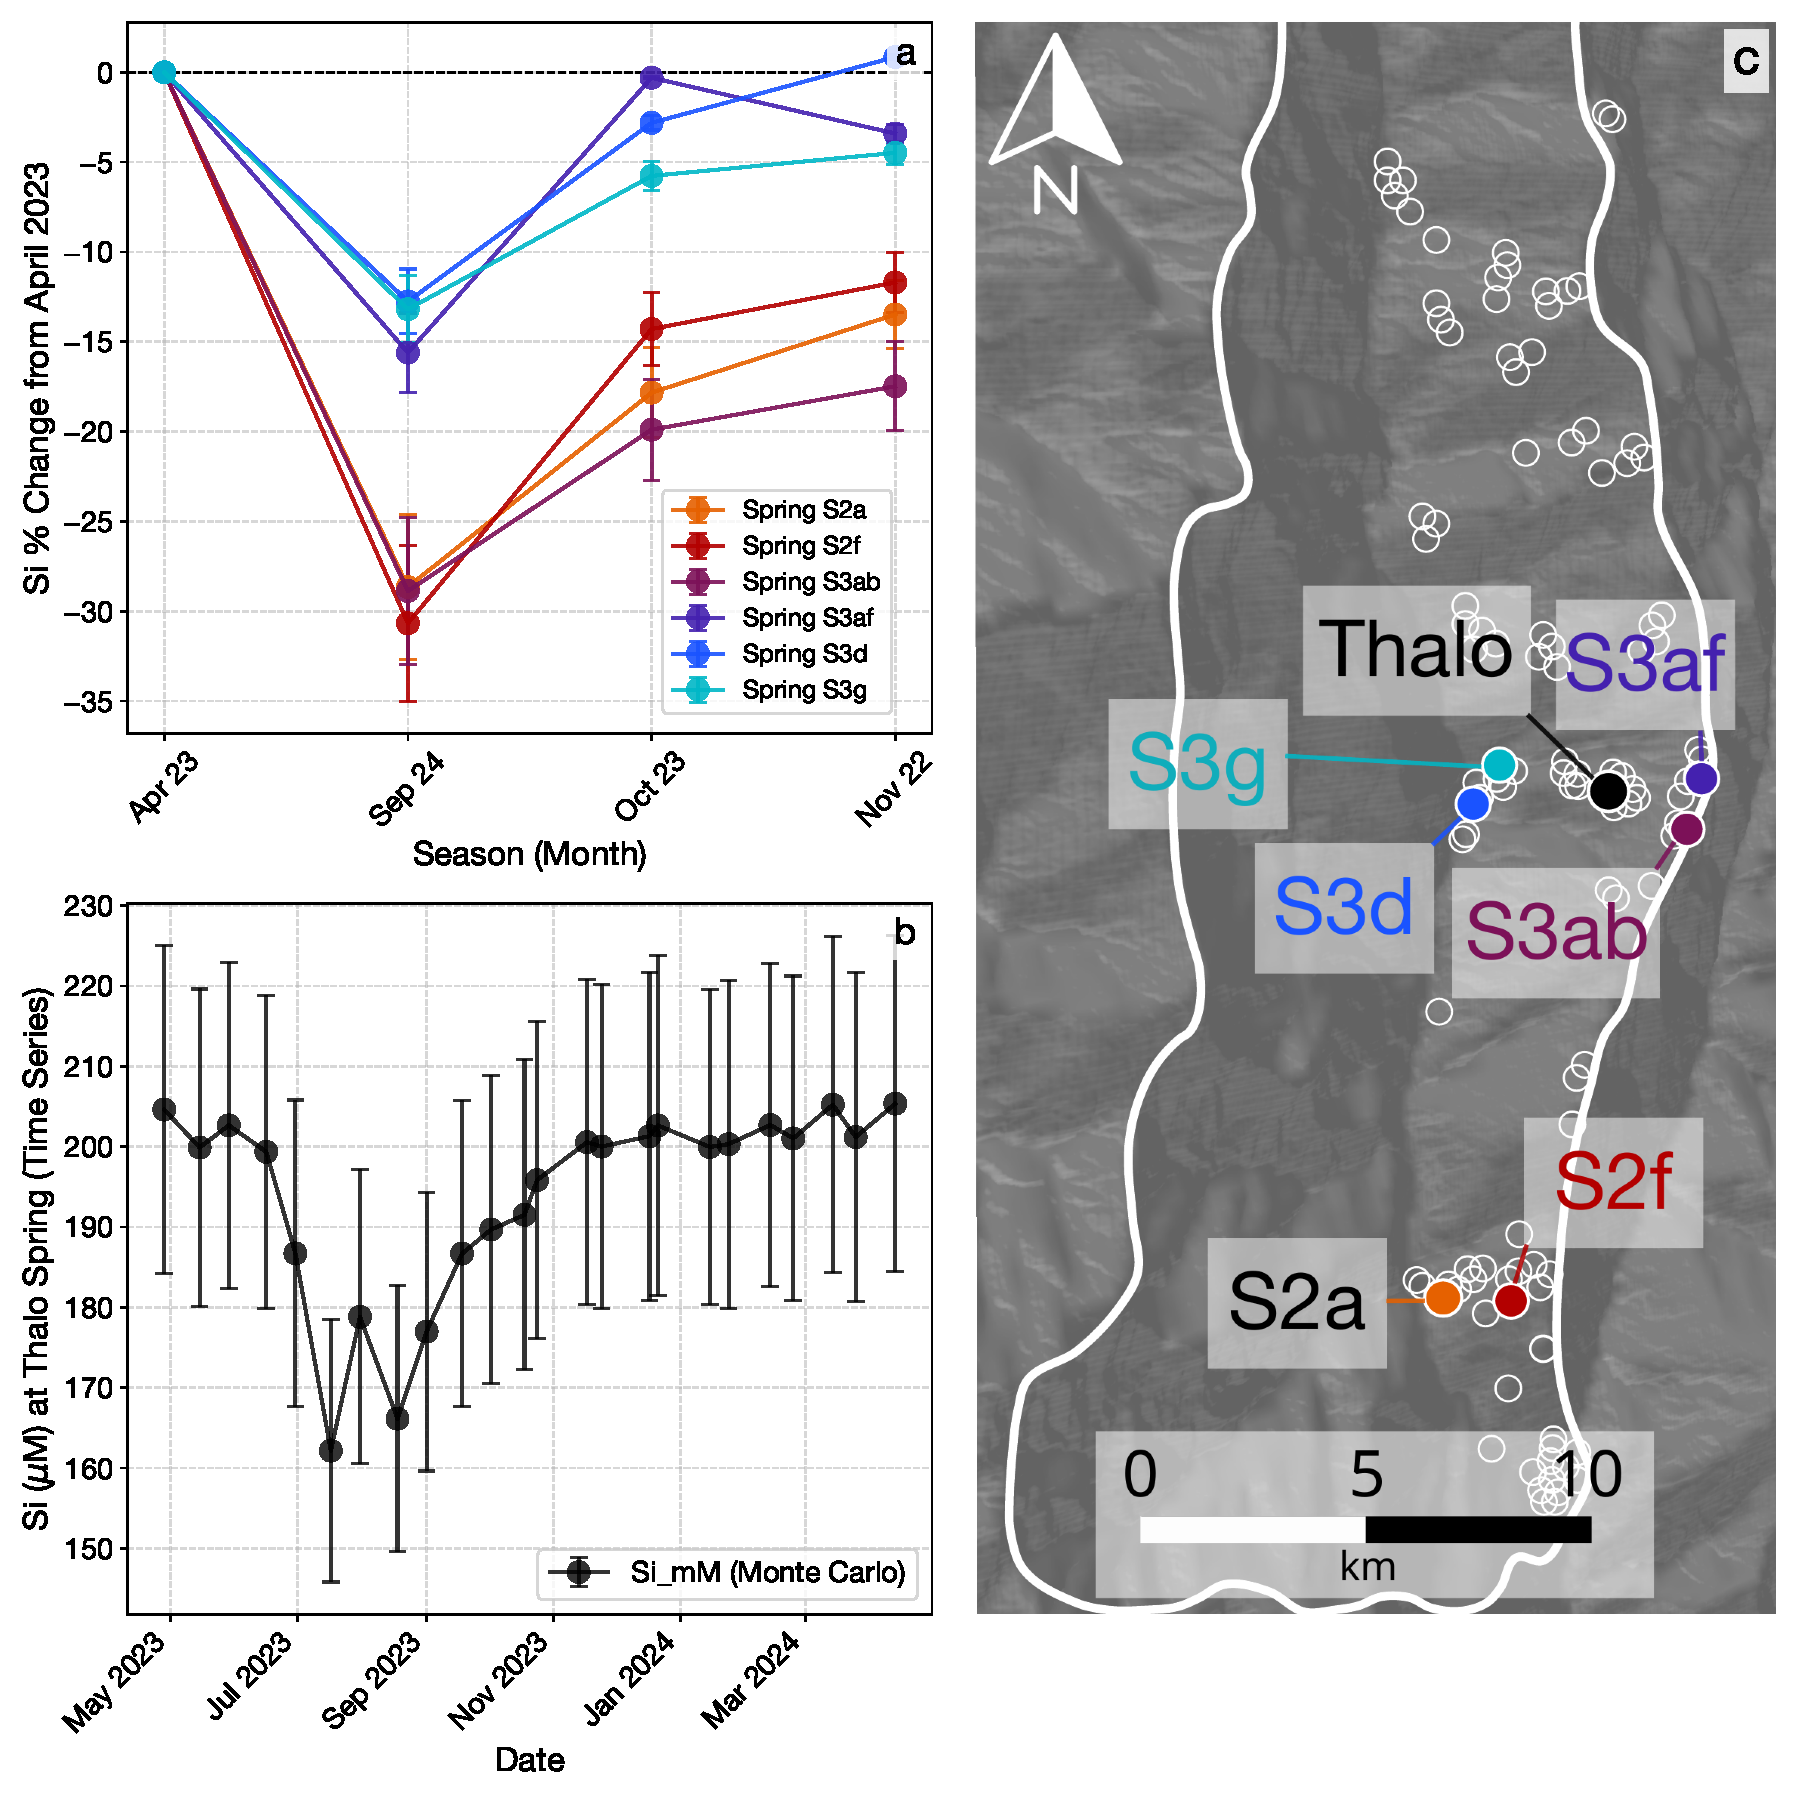
\includegraphics[width=0.9\textwidth]{Combined_Si_mM_Plots_with_Schematic.pdf}
    \caption{(a) Measured spring silica concentrations against season sampled. DSi is represented as a percentage change from April 2023, to emphasise monsoonal dilution. (b) Dissolved Silica against date sampled for time series sampled collected at a single spring, Thalo. Error bars represent monte carlo error propagation. (c) Schematic of the Melamchi catchment showing the location of springs plotted in (a) and (b).}
    \label{fig:time_series_changes}
\end{figure}

\FloatBarrier

















% \subsection{Strontium Isotope Values of Springs and Rain}



% \begin{landscape} % Start landscape mode

%     \scriptsize  % Reduce font size for better fit

%     \noindent % Avoid indentation
%     \begin{minipage}{0.48\linewidth} % First half of the landscape page

%         \begin{longtable}{l r r l r r}
%             \caption{Strontium isotope values (Part 1)} \label{tab:sr87_sr86_data1} \\
%             \hline
%             \textbf{Sample ID} & \textbf{Elevation (m)} & \textbf{pH} & \boldmath{$^{87}$Sr/$^{86}$Sr} (\textbf{2SD} $\cdot$10$^{\text{6}}$)} & \textbf{Sr ($\mu$M)} & \textbf{Cl ($\mu$M)} \\
%             \hline
%             \endfirsthead

%             \multicolumn{6}{c}{\textbf{(Continued from previous page)}} \\
%             \hline
%             \textbf{Sample ID} & \textbf{Elevation (m)} & \textbf{pH} & \boldmath{$^{87}$Sr/$^{86}$Sr} (\textbf{2SD} $\cdot$10$^{\text{6}}$)} & \textbf{Sr ($\mu$M)} & \textbf{Cl ($\mu$M)} \\
%             \hline
%             \endhead

%             \hline
%             \multicolumn{6}{r}{\textit{Continued on next column}} \\
%             \endfoot

%             \hline
%             \endlastfoot


%             \multicolumn{6}{c}{\textbf{Rain}} \\

%             NEP24-039 & 840 & 6.79 & 0.73906 \hfill (24) & 0.13 & 28.09 \\
%             NEP24-043 & 1351 & 5.82 & 0.71442 \hfill (46) & 0.01 & 3.55 \\
%             NEP24-044 & 1952 & 6.05 & 0.71352 \hfill (127) & 0.01 & 1.89 \\
%             NEP24-045 & 2644 & 5.00 & 0.71292 \hfill (73) & 0.01 & 3.21 \\
%             NEP24-046 & 2110 & 6.02 & 0.70904 \hfill (100) & 0.02 & 2.86 \\
%             NEP24-047 & 2644 & 5.74 & 0.71194 \hfill (237) & 0.01 & 0.55 \\
%             NEP24-048 & 2644 & 5.61 & 0.71182 \hfill (189) & 0.01 & 3.65 \\
%             \hline

%             \multicolumn{6}{c}{\textbf{Traverse 1}} \\
%             NEP22-1 & 871 & 7.08 & 0.74101 \hfill (29) & 0.34 & 81.09 \\
%             NEP22-2 & 890 & 7.75 & 0.74115 \hfill (22) & 0.35 & 92.95 \\
%             NEP22-80 & 1045 & 7.71 & 0.75192 \hfill (33) & 0.26 & 6.43 \\
%             NEP22-81 & 1209 & 7.89 & 0.75506 \hfill (27) & 0.21 & 10.64 \\
%             NEP22-82 & 1213 & 7.04 & 0.75517 \hfill (23) & 0.31 & 13.10 \\
%             NEP22-83 & 1245 & 6.24 & 0.75154 \hfill (27) & 0.31 & 4.31 \\
%             NEP22-84 & 1173 & 7.86 & 0.74969 \hfill (61) & 0.28 & 3.17 \\
%             NEP22-85 & 1197 & 7.56 & 0.75394 \hfill (32) & 0.16 & 2.38 \\
%             NEP22-86 & 1125 & 8.27 & 0.75957 \hfill (35) & 0.07 & 54.46 \\
%             NEP22-87 & 1268 & 6.26 & 0.74341 \hfill (25) & 0.78 & 223.01 \\
%             \hline
            
%             \multicolumn{6}{c}{\textbf{Traverse 2}} \\

%             NEP22-61 & 1528 & 5.32 & 0.74691 \hfill (62) & 0.29 & 349.74 \\
%             NEP22-62 & 1503 & 6.41 & 0.73943 \hfill (25) & 0.06 & 362.10 \\
%             NEP22-63 & 1447 & 6.73 & 0.74943 \hfill (37) & 0.47 & 152.05 \\
%             NEP22-64 & 1444 & 6.53 & 0.74872 \hfill (25) & 0.33 & 101.99 \\
%             NEP22-65 & 1430 & 6.51 & 0.74886 \hfill (30) & 0.17 & 58.79 \\
%             NEP22-66 & 1359 & 7.35 & 0.74629 \hfill (30) & 0.03 & 126.02 \\
%             NEP22-67 & 1126 & 6.83 & 0.74510 \hfill (41) & 0.48 & 235.79 \\
%             NEP22-68 & 1288 & 5.42 & 0.75696 \hfill (23) & 0.29 & 112.71 \\
%             NEP22-70 & 950 & 7.54 & 0.73128 \hfill (37) & 1.18 & 60.86 \\
%             NEP22-71 & 996 & 7.99 & 0.74253 \hfill (42) & 0.31 & 125.59 \\
%             NEP22-73 & 979 & 6.73 & 0.73191 \hfill (19) & 0.86 & 41.91 \\
%             NEP22-75 & 1054 & 6.53 & 0.73921 \hfill (71) & 0.46 & 117.33 \\
%             NEP22-76 & 1073 & 6.82 & 0.73701 \hfill (21) & 0.43 & 111.78 \\
%             NEP22-78 & 1272 & 6.74 & 0.74584 \hfill (36) & 0.17 & 40.32 \\
%             NEP22-79 & 1276 & 5.67 & 0.74752 \hfill (56) & 0.29 & 305.63 \\
%             \hline

%         \end{longtable}

%     \end{minipage} % End first column

%     \hfill % Add space between tables

%     \begin{minipage}{0.48\linewidth} % Second half of the landscape page

%         \begin{longtable}{l r r l r r}
%             \caption{Strontium isotope values (Part 2)} \label{tab:sr87_sr86_data2} \\
%             \hline
%             \textbf{Sample ID} & \textbf{Elevation (m)} & \textbf{pH} & \boldmath{$^{87}$Sr/$^{86}$Sr} (\textbf{2SD} $\cdot$10$^{\text{6}}$)} & \textbf{Sr ($\mu$M)} & \textbf{Cl ($\mu$M)} \\
%             \hline
%             \endfirsthead

%             \multicolumn{6}{c}{\textbf{(Continued from previous page)}} \\
%             \hline
%             \textbf{Sample ID} & \textbf{Elevation (m)} & \textbf{pH} & \boldmath{$^{87}$Sr/$^{86}$Sr} (\textbf{2SD} $\cdot$10$^{\text{6}}$)} & \textbf{Sr ($\mu$M)} & \textbf{Cl ($\mu$M)} \\
%             \hline
%             \endhead

%             \hline
%             \multicolumn{6}{r}{\textit{Continued on next page}} \\
%             \endfoot

%             \hline
%             \endlastfoot

%             \multicolumn{6}{c}{\textbf{Traverse 3}} \\

%             NEP22-10 & 2419 & 6.48 & 0.73918 \hfill (60) & 0.20 & 17.13 \\
%             NEP22-11 & 2419 & 6.59 & 0.73819 \hfill (20) & 0.22 & 15.76 \\
%             NEP22-12 & 2390 & 6.77 & 0.73162 \hfill (27) & 0.16 & 2.89 \\
%             NEP22-13 & 2099 & 6.76 & 0.73614 \hfill (54) & 0.25 & 9.03 \\
%             NEP22-15 & 1975 & 7.29 & 0.73841 \hfill (14) & 0.23 & 4.98 \\
%             NEP22-16 & 1967 & 7.14 & 0.73370 \hfill (22) & 0.15 & 1.05 \\
%             NEP22-17 & 2100 & 6.90 & 0.73584 \hfill (26) & 0.21 & 11.74 \\
%             NEP22-18 & 2091 & 6.98 & 0.73281 \hfill (19) & 0.38 & 8.66 \\
%             NEP22-19 & 2095 & 6.07 & 0.73594 \hfill (28) & 0.25 & 9.44 \\
%             NEP22-20 & 2104 & 7.14 & 0.73241 \hfill (34) & 0.11 & 6.87 \\
%             NEP22-42 & 1325 & 6.24 & 0.73680 \hfill (62) & 0.31 & 27.25 \\
%             NEP22-45 & 1194 & 7.57 & 0.73763 \hfill (22) & 0.32 & 23.90 \\
%             NEP22-53 & 1776 & 6.33 & 0.73720 \hfill (39) & 0.40 & 19.70 \\
%             NEP22-54 & 1781 & 6.19 & 0.73831 \hfill (18) & 0.36 & 20.39 \\
%             NEP22-55 & 1771 & 6.69 & 0.73824 \hfill (19) & 0.36 & 19.57 \\
%             NEP22-56 & 1433 & 6.86 & 0.74129 \hfill (26) & 0.42 & 23.24 \\
%             NEP22-57 & 1464 & 6.85 & 0.73240 \hfill (37) & 0.69 & 46.41 \\
%             NEP22-58 & 1447 & 7.34 & 0.73871 \hfill (19) & 0.36 & 7.57 \\
%             NEP22-59 & 1324 & 7.48 & 0.73780 \hfill (73) & 0.32 & 14.91 \\
%             NEP22-60 & 1161 & 7.04 & 0.73121 \hfill (24) & 0.38 & 22.66 \\
%             NEP24-010 & 1314 & 6.45 & 0.73689 \hfill (94) & 0.31 & 21.65 \\
%             NEP24-011 & 1319 & 7.07 & 0.73782 \hfill (29) & 0.33 & 10.92 \\
%             NEP24-014 & 2496 & 6.58 & 0.73508 \hfill (0) & 0.03 & 1.84 \\
%             NEP24-015 & 2104 & 6.10 & 0.73644 \hfill (47) & 0.20 & 7.38 \\
%             NEP24-016 & 1978 & 7.05 & 0.73360 \hfill (20) & 0.16 & 0.39 \\
%             \hline
%             \multicolumn{6}{c}{\textbf{Traverse 4}} \\

%             NEP22-46 & 2555 & 7.05 & 0.74922 \hfill (56) & 0.16 & 3.37 \\
%             NEP22-47 & 2451 & 6.65 & 0.73661 \hfill (36) & 0.19 & 7.65 \\
%             NEP22-48 & 2067 & 6.63 & 0.74727 \hfill (28) & 0.22 & 2.64 \\
%             NEP22-49 & 1968 & 6.88 & 0.73730 \hfill (28) & 0.44 & 5.12 \\
%             NEP22-50 & 1698 & 6.69 & 0.73508 \hfill (39) & 0.62 & 21.22 \\
%             NEP22-52 & 1532 & 7.00 & 0.73828 \hfill (22) & 0.18 & 7.99 \\
%             \hline
%             \multicolumn{6}{c}{\textbf{Traverse 5}} \\

%             NEP22-22 & 2755 & 6.90 & 0.73006 \hfill (20) & 0.19 & 1.94 \\
%             NEP22-23 & 2516 & 6.17 & 0.73210 \hfill (26) & 0.13 & 1.19 \\
%             NEP22-24 & 2626 & 7.16 & 0.72989 \hfill (20) & 0.19 & 5.93 \\
%             NEP22-25 & 2566 & 7.24 & 0.72999 \hfill (44) & 0.24 & 4.23 \\
%             NEP22-26 & 2577 & 6.83 & 0.73230 \hfill (22) & 0.11 & 1.73 \\
%             NEP22-27 & 3122 & 7.00 & 0.73165 \hfill (35) & 0.09 & 1.53 \\
%             NEP22-28 & 2953 & 7.22 & 0.73238 \hfill (26) & 0.11 & 1.73 \\
%             NEP22-29 & 2850 & 7.24 & 0.73218 \hfill (22) & 0.15 & 1.71 \\
%             NEP22-30 & 2760 & 6.70 & 0.73243 \hfill (24) & 0.17 & 3.08 \\
%             NEP22-31 & 2564 & 6.90 & 0.73244 \hfill (25) & 0.28 & 1.96 \\
%             NEP22-32 & 2252 & 6.27 & 0.73227 \hfill (23) & 0.26 & 11.19 \\
%             NEP22-33 & 2249 & 7.51 & 0.73166 \hfill (20) & 0.26 & 13.14 \\
%             NEP22-34 & 2240 & 7.35 & 0.73155 \hfill (56) & 0.27 & 16.81 \\
%             NEP22-35 & 2066 & 7.55 & 0.73334 \hfill (19) & 0.16 & 2.78 \\
%             NEP22-36 & 1986 & 7.84 & 0.73205 \hfill (20) & 0.27 & 3.00 \\
%             NEP22-37 & 2050 & 7.72 & 0.73280 \hfill (44) & 0.22 & 2.33 \\
%             NEP22-39 & 2524 & 7.60 & 0.73116 \hfill (22) & 0.18 & 4.51 \\

%             \hline
%         \end{longtable}

%     \end{minipage} % End first column

% \end{landscape}


% \FloatBarrier


% Radiogenic strontium isotope analyses of springs show a wide variation between different traverses. Sr isotopes were also measured for the collected rain samples, and these range from 0.70904 to 0.73906. The lowest of these rain values is close to the reported value for seawater, which is 0.70917.  